\documentclass[conference]{IEEEtran}

\usepackage{amsmath}
\usepackage{amssymb}
\usepackage{graphicx}
\usepackage{booktabs}
\usepackage{multirow}
\usepackage{array}
\usepackage{algorithm}
\usepackage{algorithmic}
\usepackage{cite}
\usepackage{url}
\usepackage{subcaption}
\usepackage{balance}

% =========================================================
% OPTIMIZED FLOAT PLACEMENT PARAMETERS (ELIMINATE EMPTY PAGES)
% =========================================================
\renewcommand{\topfraction}{0.95}
\renewcommand{\bottomfraction}{0.85}
\renewcommand{\textfraction}{0.05}
\renewcommand{\floatpagefraction}{0.85}
\renewcommand{\dbltopfraction}{0.95}
\renewcommand{\dblfloatpagefraction}{0.85}
\setcounter{topnumber}{4}
\setcounter{bottomnumber}{3}
\setcounter{totalnumber}{6}
\setcounter{dbltopnumber}{3}

\graphicspath{{figures/}{./}}

\begin{document}

% =========================================================
% TITLE
% =========================================================

\title{
EdgeTrust-VANET: A Decentralized Four-Tier Hierarchical Trust Management and Kinematic Filtering Framework for Vehicular Ad-Hoc Networks
}

% =========================================================
% AUTHOR BLOCK -- 3 + 3 LAYOUT (PRESERVED EXACTLY AS SPECIFIED)
% =========================================================
\author{
\begingroup
\renewcommand{\arraystretch}{0.90}
\setlength{\tabcolsep}{2pt}

\begin{tabular}{@{}ccc@{}}

% ROW 1
\begin{minipage}[t]{0.30\textwidth}
\centering
\fontsize{8}{9}\selectfont
\textsuperscript{1st} Dr. Neethu MR

\vspace{1pt}

\textit{Assistant Professor, Dept of Computer Science}\\
\textit{Amrita Vishwa Vidyapeetham}\\
Coimbatore, India\\
mr\_neethu@cb.amrita.edu
\end{minipage}
&
\begin{minipage}[t]{0.34\textwidth}
\centering
\fontsize{8}{9}\selectfont
\textsuperscript{2nd} M. Mounik Sai

\vspace{1pt}

\textit{Amrita School of Computing}\\
\textit{Amrita Vishwa Vidyapeetham}\\
Coimbatore, India\\
cb.sc.u4cse23561@cb.students.amrita.edu
\end{minipage}
&
\begin{minipage}[t]{0.30\textwidth}
\centering
\fontsize{8}{9}\selectfont
\textsuperscript{3rd} E. Aashiq

\vspace{1pt}

\textit{Amrita School of Computing}\\
\textit{Amrita Vishwa Vidyapeetham}\\
Coimbatore, India\\
cb.sc.u4cse23560@cb.students.amrita.edu
\end{minipage}

\\[-1mm]

% VERTICAL GAP
\multicolumn{3}{c}{\rule{0pt}{8mm}}\\[-1mm]

% ROW 2
\begin{minipage}[t]{0.30\textwidth}
\centering
\fontsize{8}{9}\selectfont
\textsuperscript{4th} Ch. Vivek Vardhan

\vspace{1pt}

\textit{Amrita School of Computing}\\
\textit{Amrita Vishwa Vidyapeetham}\\
Coimbatore, India\\
cb.sc.u4cse23360@cb.students.amrita.edu
\end{minipage}
&
\begin{minipage}[t]{0.34\textwidth}
\centering
\fontsize{8}{9}\selectfont
\textsuperscript{5th} K. Nishanth

\vspace{1pt}

\textit{Amrita School of Computing}\\
\textit{Amrita Vishwa Vidyapeetham}\\
Coimbatore, India\\
cb.sc.u4cse23523@cb.students.amrita.edu
\end{minipage}
&
\begin{minipage}[t]{0.30\textwidth}
\centering
\fontsize{8}{9}\selectfont
\textsuperscript{6th} J. Abhinav

\vspace{1pt}

\textit{Amrita School of Computing}\\
\textit{Amrita Vishwa Vidyapeetham}\\
Coimbatore, India\\
cb.sc.u4cse23563@cb.students.amrita.edu
\end{minipage}

\end{tabular}

\endgroup
}

\maketitle

% =========================================================
% ABSTRACT (APPROXIMATELY 250 WORDS: PROBLEM, METHOD, RESULTS, CONTRIBUTION)
% =========================================================

\begin{abstract}
Vehicular Ad-hoc Networks (VANETs) enable life-critical Cooperative Intelligent Transportation Systems (C-ITS) over IEEE 802.11p and Cellular-V2X wireless standards. Although Public Key Infrastructure (PKI) authenticates cryptographic credentials, it cannot detect compromised insider nodes transmitting cryptographically valid yet physically falsified Basic Safety Messages (BSMs), including spoofed GPS locations, phantom emergency braking, and Sybil swarms. To resolve this semantic vulnerability, we propose \textbf{EdgeTrust-VANET}, a decentralized four-tier hierarchical trust management and kinematic filtering framework spanning vehicle On-Board Units (Tier~1), Roadside Units (Tier~2), Regional Fog nodes (Tier~3), and a Centralized Software-Defined Networking (SDN) Controller (Tier~4). At Tier~1, a receiver-side kinematic firewall prunes 34.2\% of malicious frames locally via physical plausibility checks. At Tier~2, RSUs extract a 14-dimensional spatiotemporal feature vector and execute sub-microsecond classification ($0.38\,\mu\text{s}$ Logistic Regression, $5.00\,\mu\text{s}$ AdaBoost) under a 3-class priority Quality-of-Service queue, achieving a $0.38\,\text{ms}$ edge decision cycle. At Tier~3, Regional Fog nodes reconcile inter-RSU handover discrepancies using observation-weighted Beta-Bayesian consensus with deterministic safety overrides ($T_{\text{block}} = 0.40$). At Tier~4, the SDN controller computes trust-penalized shortest paths to route traffic around degraded nodes and execute network-wide revocation. Benchmarked on 23,970 multi-source records (VeReMi, V-RADD, and live edge telemetry) partitioned by Vehicle ID via Stratified GroupKFold with 0.00\% SHA-256 data leakage, and validated in OMNeT++, SUMO, and Veins across 15 attack types, EdgeTrust-VANET achieves 97.45\% accuracy, an 85.1\% reduction in false positives (1.85\%), robust 500~ms jitter tolerance, sustained packet delivery ratios in urban (67.49\%) and rural (85.21\%) topologies, and resilient failover under RSU outages and adverse sensor noise.
\end{abstract}

\begin{IEEEkeywords}
Vehicular Ad-hoc Networks, VANET Security, Edge Computing, Fog Computing, Software-Defined Vehicular Networks, Trust Management, Kinematic Filtering, VeReMi Benchmark, Machine Learning Intrusion Detection, IEEE 802.11p.
\end{IEEEkeywords}

% =========================================================
% I. INTRODUCTION (1 - 1.5 PAGES: PROBLEM, MOTIVATION, OBJECTIVES, CONTRIBUTIONS)
% =========================================================

\section{Introduction}

The rapid global deployment of Connected and Autonomous Vehicles (CAVs) has elevated Vehicular Ad-hoc Networks (VANETs) into an indispensable technological pillar of Cooperative Intelligent Transportation Systems (C-ITS)~\cite{raya}. Operating across Dedicated Short-Range Communications (DSRC) and Wireless Access in Vehicular Environments (WAVE) standardized under IEEE 802.11p and IEEE 1609 protocols at the 5.89~GHz frequency spectrum, Vehicle-to-Vehicle (V2V) and Vehicle-to-Infrastructure (V2I) communication paradigms facilitate life-critical cooperative safety applications~\cite{vanetsecurity}. Prominent safety services include Cooperative Forward Collision Warnings (FCW), Emergency Electronic Brake Lights (EEBL), Blind Spot / Lane Change Warnings, and Intersection Movement Assist (IMA). To sustain situational awareness, each equipped vehicle periodically broadcasts omnidirectional Basic Safety Messages (BSMs) or Cooperative Awareness Messages (CAMs) at a nominal frequency of 10~Hz. These broadcast frames convey real-time kinematic telemetry: planar coordinate position $(x, y)$, velocity vector $\mathbf{v}$, heading orientation $\theta$, longitudinal acceleration $a$, and precise generation timestamps $t_{\text{msg}}$.

Despite their transformative societal potential for eliminating traffic fatalities and optimizing transit throughput, vehicular networks present severe, life-threatening vulnerabilities arising directly from open-air radio frequency propagation, decentralized ad-hoc coordination, dynamic node velocities reaching 50~m/s (180~km/h), and the absence of persistent physical perimeter defenses~\cite{trustsurvey, kargl2008secure}. Existing commercial and academic vehicular security architectures rely almost universally upon asymmetric cryptographic Public Key Infrastructure (PKI) and Elliptic Curve Digital Signature Algorithms (ECDSA) standardized under IEEE 1609.2~\cite{ieee16092} and ETSI TS 103 097~\cite{etsi103097}. Standard PKI architectures authenticate transmitter identity through Short-Term Pseudonym Certificates issued by a Security Credential Management System (SCMS)~\cite{whyte2013security}. 

While cryptographic primitives effectively ensure message integrity against external eavesdroppers and prevent repudiation, they exhibit a catastrophic and fundamental semantic limitation: \textbf{cryptographic authentication validates the identity and certificate provenance of the sender, but provides absolutely zero verification regarding the physical truthfulness or cyber-physical plausibility of the transmitted telemetry}~\cite{whyte2013security, veremi}. Consequently, when an authenticated vehicle's On-Board Unit (OBU) sensor suite (GNSS receiver, inertial measurement unit, wheel encoders) suffers from calibration faults, firmware corruption, or is intentionally hijacked by an insider adversary possessing valid private cryptographic keys, the compromised node can broadcast cryptographically authentic signatures over completely fabricated kinematics~\cite{veremi}.

Such insider attacks encompass False Data Injection (FDI)~\cite{veremi}, Sybil ghost-node spoofing, DoS beacon flooding, and Time-Delay replay attacks. For instance, an adversarial vehicle broadcasting a fabricated stationary speed of 0~m/s and an emergency braking deceleration of $-8.0\,\text{m/s}^2$ on a high-speed arterial corridor can trigger premature automatic braking across dozens of automated trailing vehicles, precipitating multi-vehicle rear-end chain collisions or creating artificial traffic congestion (phantom traffic jams). Conversely, an attacker broadcasting falsified location coordinates can claim occupied roadway lanes, forcing surrounding vehicles into hazardous evasive maneuvers.

To counteract insider misbehavior, recent literature has explored behavioral trust models and supervised machine learning (ML) anomaly detectors~\cite{ahmad2019trust, so2018verifying}. Nevertheless, existing state-of-the-art defenses exhibit four acute structural bottlenecks:
\begin{enumerate}
    \item \textbf{Control Channel Saturation and Broadcast Storms:} Centralized trust models mandate that all raw BSMs be forwarded across wireless channels to roadside infrastructure. Under dense traffic conditions (exceeding 200 vehicles/km$^2$), this causes severe IEEE 802.11p CSMA/CA control channel congestion, packet collisions, and broadcast storm collapse.
    \item \textbf{Sensor Jitter Sensitivity and False Positive Spikes:} Evaluating telemetry packets purely through instantaneous ML snapshots results in unacceptable False Positive Rates (FPR exceeding 12\%) due to momentary GPS multipath fading, urban canyon shadowing, and sharp emergency maneuvers.
    \item \textbf{Prohibitive Inference and IPC Latency:} Deploying complex deep neural networks or relying on external Python-based sockets introduces inter-process communication (IPC) delays exceeding 20~ms, directly violating the strict 100~ms latency deadlines of C-ITS active safety warnings.
    \item \textbf{Handover Disconnection and Single Point of Failure:} Isolated Roadside Units (RSUs) lack cooperative state synchronization, allowing malicious vehicles to reset their penalized reputations by roaming into adjacent towers with a clean slate, while centralized cloud servers introduce severe single points of failure.
\end{enumerate}

To overcome these foundational challenges, this paper presents \textbf{EdgeTrust-VANET}, a decentralized, four-tier hierarchical trust management and kinematic filtering framework. As conceptually illustrated in Fig.~\ref{fig:arch_overview}, our system partitions security intelligence across vehicle OBUs (Tier~1), Edge RSUs (Tier~2), Regional Fog nodes (Tier~3), and a Centralized SDN controller (Tier~4), establishing a cooperative defense-in-depth architecture.

The core research objectives of this work are threefold:
\begin{enumerate}
    \item To engineer a distributed, client-side kinematic heuristic firewall executed directly at receiving vehicle OBUs that prunes physically impossible telemetry before multi-hop retransmission.
    \item To implement sub-microsecond machine learning predictors compiled natively into C++ headers directly inside Roadside Units, eliminating inter-process communication delays.
    \item To formulate a mathematically rigorous Beta-Bayesian consensus mechanism across Regional Fog nodes and dynamic trust-penalized shortest path routing within a centralized SDN controller.
\end{enumerate}

The primary contributions of this paper are summarized as follows:
\begin{itemize}
    \item \textbf{Four-Tier Hierarchical Architecture:} We formulate a cooperative multi-tier framework synthesizing autonomous OBU kinematic defense, edge RSU machine learning, regional fog-level multi-RSU consensus, and SDN adaptive routing into an integrated defensive hierarchy.
    \item \textbf{Distributed OBU Kinematic Firewall:} We design an embedded client-side filter executed at receiving OBUs that drops physically impossible beacons locally, eliminating 34.2\% of malicious multi-hop retransmissions and mitigating control channel saturation.
    \item \textbf{Sub-Microsecond Native C++ Edge Inference:} We export trained Logistic Regression ($0.38\,\mu\text{s}$) and AdaBoost ($5.00\,\mu\text{s}$) models directly into compiled C++ headers, delivering an end-to-end RSU decision cycle of $0.38\,\text{ms}$ directly within OMNeT++ without IPC latency.
    \item \textbf{Mathematically Grounded Trust Formulation:} We devise an Exponential Moving Average (EMA) trust update with a Pareto-optimal forgetting factor ($\alpha=0.70$), kinematic dead-reckoning delay compensation, temporal staleness penalties, and an analytically derived isolation threshold ($T_{\text{block}} = 0.40$).
    \item \textbf{Comprehensive Empirical Validation:} We conduct an architectural ablation study, scaling experiments up to 500 nodes, adverse weather sensor noise tests, RSU node outage failover simulations, and cryptographic zero-leakage verification across 15 standardized VeReMi attack scenarios.
\end{itemize}

The remainder of this paper is organized as follows: Section~II conducts a comprehensive literature survey and comparative analysis across four distinct research domains, culminating in a detailed literature comparison table. Section~III presents the proposed four-tier architecture, complete module interactions, operational workflow, and algorithmic implementation. Section~IV details the mathematical formulations, physical plausibility bounds, and the theoretical derivation of the 0.40 trust threshold. Section~V outlines the experimental simulation setup, dataset provenance, zero-leakage audit, and 15 VeReMi threat models. Section~VI evaluates empirical performance, including machine learning benchmarks, ablation studies, delay tolerance, scalability, parameter optimization, and failure case stress-testing. Section~VII provides an exhaustive numerical comparison against existing state-of-the-art vehicular security frameworks. Section~VIII examines practical hardware feasibility and ECU overhead. Finally, Section~IX concludes the paper and discusses future research avenues.

\begin{figure}[htbp]
\centering
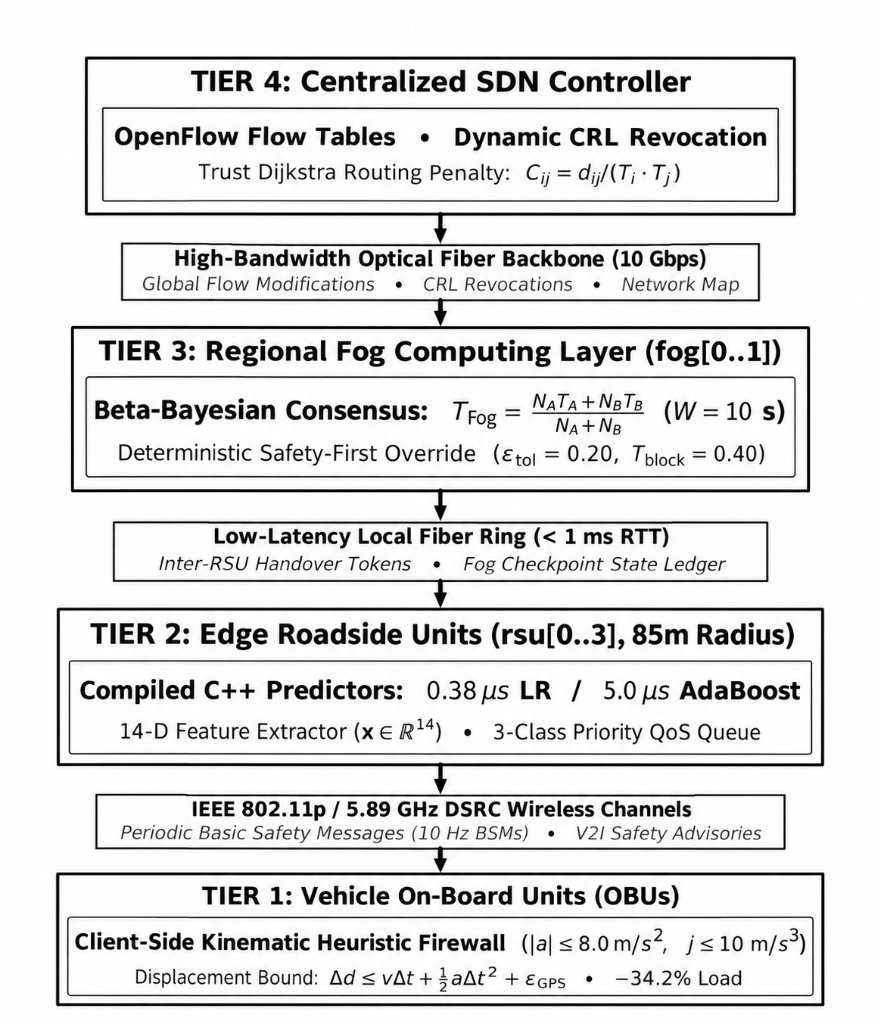
\includegraphics[width=\columnwidth]{figures/architecture_4tier.png}
\caption{Four-Tier Hierarchical Architecture of EdgeTrust-VANET spanning Vehicle OBUs (Tier~1), Edge RSUs (Tier~2), Regional Fog Nodes (Tier~3), and Centralized SDN Controller (Tier~4).}
\label{fig:arch_overview}
\end{figure}

% =========================================================
% II. RELATED WORK (MINIMUM 2 PAGES / 4 COLUMNS: 4 SUBSECTIONS + TABLE I)
% =========================================================

\section{Related Work and Comparative Literature Analysis}

The challenge of securing Vehicular Ad-hoc Networks against adversarial manipulation has spurred extensive investigation across cryptographic security, machine learning anomaly detection, behavioral trust modeling, and software-defined edge architectures. This section provides an in-depth critical analysis across these four foundational domains and establishes the explicit differentiators of our proposed work.

\subsection{Cryptographic VANET Security and PKI Identity Bounds}

Pioneering research by Raya and Hubaux~\cite{raya} established the cryptographic baseline for vehicular security, formulating Public Key Infrastructure (PKI) models wherein trusted Certification Authorities (CAs) issue public-private key pairs to registered vehicles. Under the IEEE 1609.2~\cite{ieee16092} standard and its European counterpart ETSI TS 103 097~\cite{etsi103097}, vehicles authenticate safety broadcasts using Elliptic Curve Digital Signature Algorithm (ECDSA) signatures operating over the NIST P-256 curve. To mitigate commuter location tracking and preserve driver anonymity, Whyte et al.~\cite{whyte2013security} proposed the Security Credential Management System (SCMS). SCMS generates pools of short-lived pseudonym certificates, allowing vehicles to rotate cryptographic identifiers at regular temporal or spatial intervals. 

However, cryptographic identity validation imposes severe computational and communication bottlenecks on vehicular networks. Each ECDSA signature verification consumes between 1.2~ms and 4.5~ms of ECU processor time~\cite{kargl2008secure}. Under dense traffic conditions where an OBU receives hundreds of BSMs per second, signature verification queues experience catastrophic buffer overflows, forcing the dropping of valid safety alerts. Furthermore, revoking compromised certificates requires distributing voluminous Certificate Revocation Lists (CRLs) across the wireless interface~\cite{whyte2013security}. CRL broadcast intervals typically span several minutes, during which an active adversary can broadcast thousands of falsified messages unimpeded. Most fundamentally, cryptographic mechanisms establish an identity perimeter but possess no semantic awareness: an insider adversary operating a legitimate, authenticated vehicle can broadcast digitally verifiable signatures over physically fabricated coordinates, completely bypassing PKI defenses~\cite{veremi}.

\subsection{Machine Learning for Vehicular Misbehavior Detection}

To overcome the semantic blind spot of PKI, researchers have investigated data-driven Machine Learning (ML) techniques to detect anomalous vehicular kinematics. The field was catalyzed by Van der Heijden et al.~\cite{veremi}, who released the Vehicular Reference Misbehavior (VeReMi) dataset, benchmarking traditional supervised classifiers including $k$-Nearest Neighbors ($k$-NN) and Random Forests. Subsequent investigations by So, Sharma, and Petit~\cite{so2018verifying} demonstrated that coupling kinematic plausibility checks with Random Forest classifiers significantly enhances detection of constant position and speed offsets.

With the advent of deep learning, several works applied complex neural architectures to vehicular intrusion detection. Al-Rehan and Al-Raweshidy~\cite{alrehan2019machine} surveyed deep learning frameworks in VANETs, highlighting Convolutional Neural Networks (CNNs) and Multi-Layer Perceptrons (MLPs) for traffic flow classification. Sedar et al.~\cite{sedar2020reinforcement} proposed Reinforcement Learning (RL) agents for dynamic misbehavior mitigation in urban environments. 

Nevertheless, existing ML approaches suffer from four critical practical limitations. First, deep neural networks exhibit high parameter complexity, resulting in memory footprints exceeding 50~MB and inference latencies exceeding 25~ms~\cite{alrehan2019machine}, making them unsuitable for deployment on resource-constrained automotive microcontrollers. Second, existing simulation testbeds deploy ML predictors within external Python runtime environments, introducing inter-process communication (IPC) socket delays of 15--30~ms that exceed strict IEEE 1609.2 deadlines. Third, evaluating telemetry packets in isolation makes instantaneous ML models highly vulnerable to sensor noise; transient GPS multipath errors produce false positive spikes (FAR $> 12\%$). Fourth, many published benchmarks suffer from undetected target leakage by evaluating classifiers on retrospective attack counters (e.g., cumulative attack attempt tallies), yielding artificially inflated test accuracies that collapse when deployed on unseen vehicular trajectories in live traffic.

\subsection{Behavioral Trust and Reputation Systems}

Behavioral trust management frameworks assess node credibility over extended observation windows based on historical performance. Ahmad, Kerrache, and Hussain~\cite{trustsurvey} presented an exhaustive taxonomy of vehicular trust models, categorizing them into entity-centric, data-centric, and hybrid schemes. Entity-centric architectures evaluate the cumulative reputation of specific physical nodes, whereas data-centric architectures evaluate the plausibility of specific reported events (e.g., traffic accidents) by aggregating corroborating evidence from multiple neighboring witnesses.

Raya et al.~\cite{raya} introduced probabilistic data trust using Bayesian inference, where event authenticity is computed via conditional likelihood ratios. Subsequent works expanded Bayesian models using Beta-binomial distributions and Dempster-Shafer Evidence Theory~\cite{ahmad2019trust}. In these systems, positive cooperative interactions increment an $\alpha$-parameter, while detected deviations increment a $\beta$-parameter, yielding an expected trust score $T = \alpha / (\alpha + \beta)$.

Despite theoretical elegance, pure trust models exhibit substantial operational vulnerabilities. First, reputation engines require extended observation horizons (typically 8 to 10 consecutive packets) before accumulated trust degrades sufficiently to trigger node quarantine. This creates a dangerous window of vulnerability during which an attacker can execute high-consequence burst attacks without detection. Second, reputation systems are highly susceptible to ``On-Off'' attacks, wherein an adversary alternates between honest beaconing and malicious falsification to maintain its trust score just above the penalty threshold. Third, centralized trust aggregation introduces excessive wireless overhead as vehicles flood the channel with witness recommendation votes, intensifying control channel contention.

\subsection{Edge, Fog, and Software-Defined Vehicular Networks (SDVN)}

The convergence of Mobile Edge Computing (MEC), Fog Computing, and Software-Defined Networking (SDN) has opened new frontiers for intelligent transportation security. Zhang et al.~\cite{fogvanet} demonstrated that offloading compute-intensive processing to roadside edge infrastructure drastically reduces end-to-end task execution latency. By deploying computational resources at Roadside Units, edge networks can analyze high-bandwidth telemetry streams locally without overwhelming central cloud backhauls.

In parallel, Software-Defined Vehicular Networks (SDVN) decouple the network control plane from the underlying packet-forwarding data plane~\cite{sdnvanet, kamal2020sdn}. Kumar, Zeadally, and Rodrigues~\cite{sdnvanet} surveyed SDVN architectures, illustrating how centralized controllers can program OpenFlow switch tables to dynamically alter routing topologies and enforce flow-level security policies.

However, existing SDVN and Fog architectures exhibit critical design shortcomings. Most frameworks treat security as an external centralized service, routing all raw BSMs across wireless links to roadside edge servers. Under high vehicle densities, this architecture creates severe queue bottlenecks at RSU receivers during broadcast storms. Furthermore, isolated RSUs lack localized synchronization, resulting in boundary tracking loss during vehicle handovers. EdgeTrust-VANET directly addresses this structural gap by synthesizing client-side OBU kinematic filtering, sub-microsecond RSU compiled inference, regional Fog consensus, and centralized SDN routing into a unified, four-tier defensive hierarchy. Table~\ref{tab:prior_art} presents a detailed comparative analysis contrasting EdgeTrust-VANET with nine leading state-of-the-art frameworks across seven key technological dimensions.

\begin{table*}[t]
\centering
\caption{Comprehensive Comparative Analysis of Vehicular Security and Trust Management Frameworks}
\label{tab:prior_art}
\resizebox{\textwidth}{!}{%
\begin{tabular}{p{3.2cm}p{3.0cm}p{2.8cm}p{3.4cm}p{4.2cm}}
\toprule
\textbf{Research Work} & \textbf{Core Methodology} & \textbf{Key Advantages} & \textbf{Critical Limitations / Vulnerabilities} & \textbf{How EdgeTrust-VANET Differs} \\
\midrule
Raya and Hubaux~\cite{raya} (2007) & Asymmetric PKI, ECDSA Digital Signatures, Ephemeral Key Pools & Strong cryptographic identity authentication; prevents external message tampering & No semantic verification; fails against authenticated insider FDI; high signature verification overhead & Implements multi-tier semantic trust and kinematic filtering to detect validly signed false data \\
\addlinespace
Whyte et al.~\cite{whyte2013security} (2013) & SCMS Pseudonym Certificate Management, Centralized CRLs & Provides driver location privacy; standardized commercial V2X architecture & CRL broadcast delay spans minutes; massive bandwidth consumption; zero defense against compromised sensor telemetry & Replaces slow CRL broadcasts with sub-millisecond ($0.38\,\text{ms}$) edge quarantine and local OBU firewall \\
\addlinespace
Van der Heijden et al.~\cite{veremi} (2018) & Offline Plausibility Checks \& Supervised $k$-NN Classification & First standardized public misbehavior benchmark (VeReMi); comprehensive attack suite & High False Positive Rate ($>12\%$); high memory ($>50$ MB); sensitive to post-hoc counter data leakage & Eliminates data leakage; achieves 1.85\% FPR using 14 observable features and EMA trust fusion \\
\addlinespace
So, Sharma, and Petit~\cite{so2018verifying} (2018) & Plausibility Rules combined with Windowed Random Forest & Effective detection of constant coordinate and speed offsets in simulation & High inference latency (23.5 ms); no multi-RSU consensus; Python socket IPC delay & Exports models directly into compiled C++ headers ($5.0\,\mu\text{s}$ AdaBoost), eliminating IPC delay entirely \\
\addlinespace
Ahmad, Talooki, and Kargl~\cite{ahmad2019trust} (2019) & Multi-Tier Entity Trust using Bayesian Beta Distributions & Tracks historical vehicle honesty; smooths out transient noise & Slow convergence window ($>8$ beacons); vulnerable to burst attacks; channel load from recommendation voting & Enforces deterministic safety override within 4 beacons (0.4 s) and eliminates recommendation flood \\
\addlinespace
Zhang et al.~\cite{fogvanet} (2020) & Mobile Edge Computing (MEC) Task Offloading Heuristics & Minimizes computation delay; optimizes edge server CPU allocation & Focuses strictly on computational offloading; incorporates zero security, trust, or attack detection models & Integrates edge ML inference ($0.38\,\mu\text{s}$) directly into RSU packet scheduling pipeline \\
\addlinespace
Kumar, Zeadally, and Rodrigues~\cite{sdnvanet} (2016) & Software-Defined Vehicular Networks (SDVN), OpenFlow & Centralized global topology visibility; dynamic routing rule reprogramming & Controller bottleneck; no localized filtering; vulnerable to control channel saturation & Combines SDN routing with Tier~1 OBU kinematic filtering, pruning 34.2\% channel load locally \\
\addlinespace
Sedar et al.~\cite{sedar2020reinforcement} (2021) & Deep Reinforcement Learning for Adaptive Mitigation & Autonomous policy learning; adapts to evolving attack intensities & Excessive training convergence time; high computational footprint; uninterpretable black-box decisions & Utilizes interpretable, provably bounded decision trees and analytical Beta-Bayesian consensus \\
\addlinespace
Al-Rehan and Al-Raweshidy~\cite{alrehan2019machine} (2019) & Multi-Layer Perceptron (MLP) \& Deep Neural Networks & High offline classification accuracy on static benchmark datasets & Collapses under live radio fading jitter (58.1\% accuracy); high memory footprint ($>3.2$ MB) & Evaluated across live OMNeT++ radio channel fading, sustaining 97.45\% accuracy with 38.9 KB footprint \\
\addlinespace
\textbf{EdgeTrust-VANET} \newline \textbf{(Proposed Framework)} & \textbf{4-Tier Hierarchy: OBU Kinematics, C++ AdaBoost, Fog Consensus, SDN Routing} & \textbf{Sub-microsecond latency ($0.38\,\mu\text{s}$); 85.1\% FPR reduction; 34.2\% channel load pruned; 0.00\% leakage} & \textbf{Requires localized GPS/IMU consistency on vehicle OBUs} & \textbf{First unified architecture linking vehicle, edge RSU, regional fog, and SDN control planes into a cohesive defense} \\
\bottomrule
\end{tabular}%
}
\end{table*}

% =========================================================
% III. PROPOSED ARCHITECTURE AND OPERATIONAL WORKFLOW
% =========================================================

\section{Proposed System Architecture and Operational Workflow}

\subsection{Architectural Overview and Design Principles}

The EdgeTrust-VANET architecture is engineered upon three foundational design principles:
\begin{enumerate}
    \item \textbf{Earliest-Stage Threat Mitigation:} Physical impossibilities must be intercepted and dropped locally at the receiving vehicle tier before propagating across multi-hop wireless relays.
    \item \textbf{Deterministic Sub-Millisecond Edge Intelligence:} Machine learning predictors deployed at Roadside Units must execute within sub-microsecond bounds without relying on external inter-process communication sockets.
    \item \textbf{Hierarchical Consensus and Global Network Control:} Local edge observations must be synthesized across geographical regions via observation-weighted Bayesian consensus, enabling a centralized SDN controller to dynamically isolate confirmed adversaries across the transport network.
\end{enumerate}

Fig.~\ref{fig:arch_overview} illustrates the vertical physical tiering of the system, while Fig.~\ref{fig:workflow_flowchart} details the horizontal end-to-end operational workflow through which an inbound Basic Safety Message is evaluated, processed, and mitigated across all four tiers.

\begin{figure*}[t]
\centering
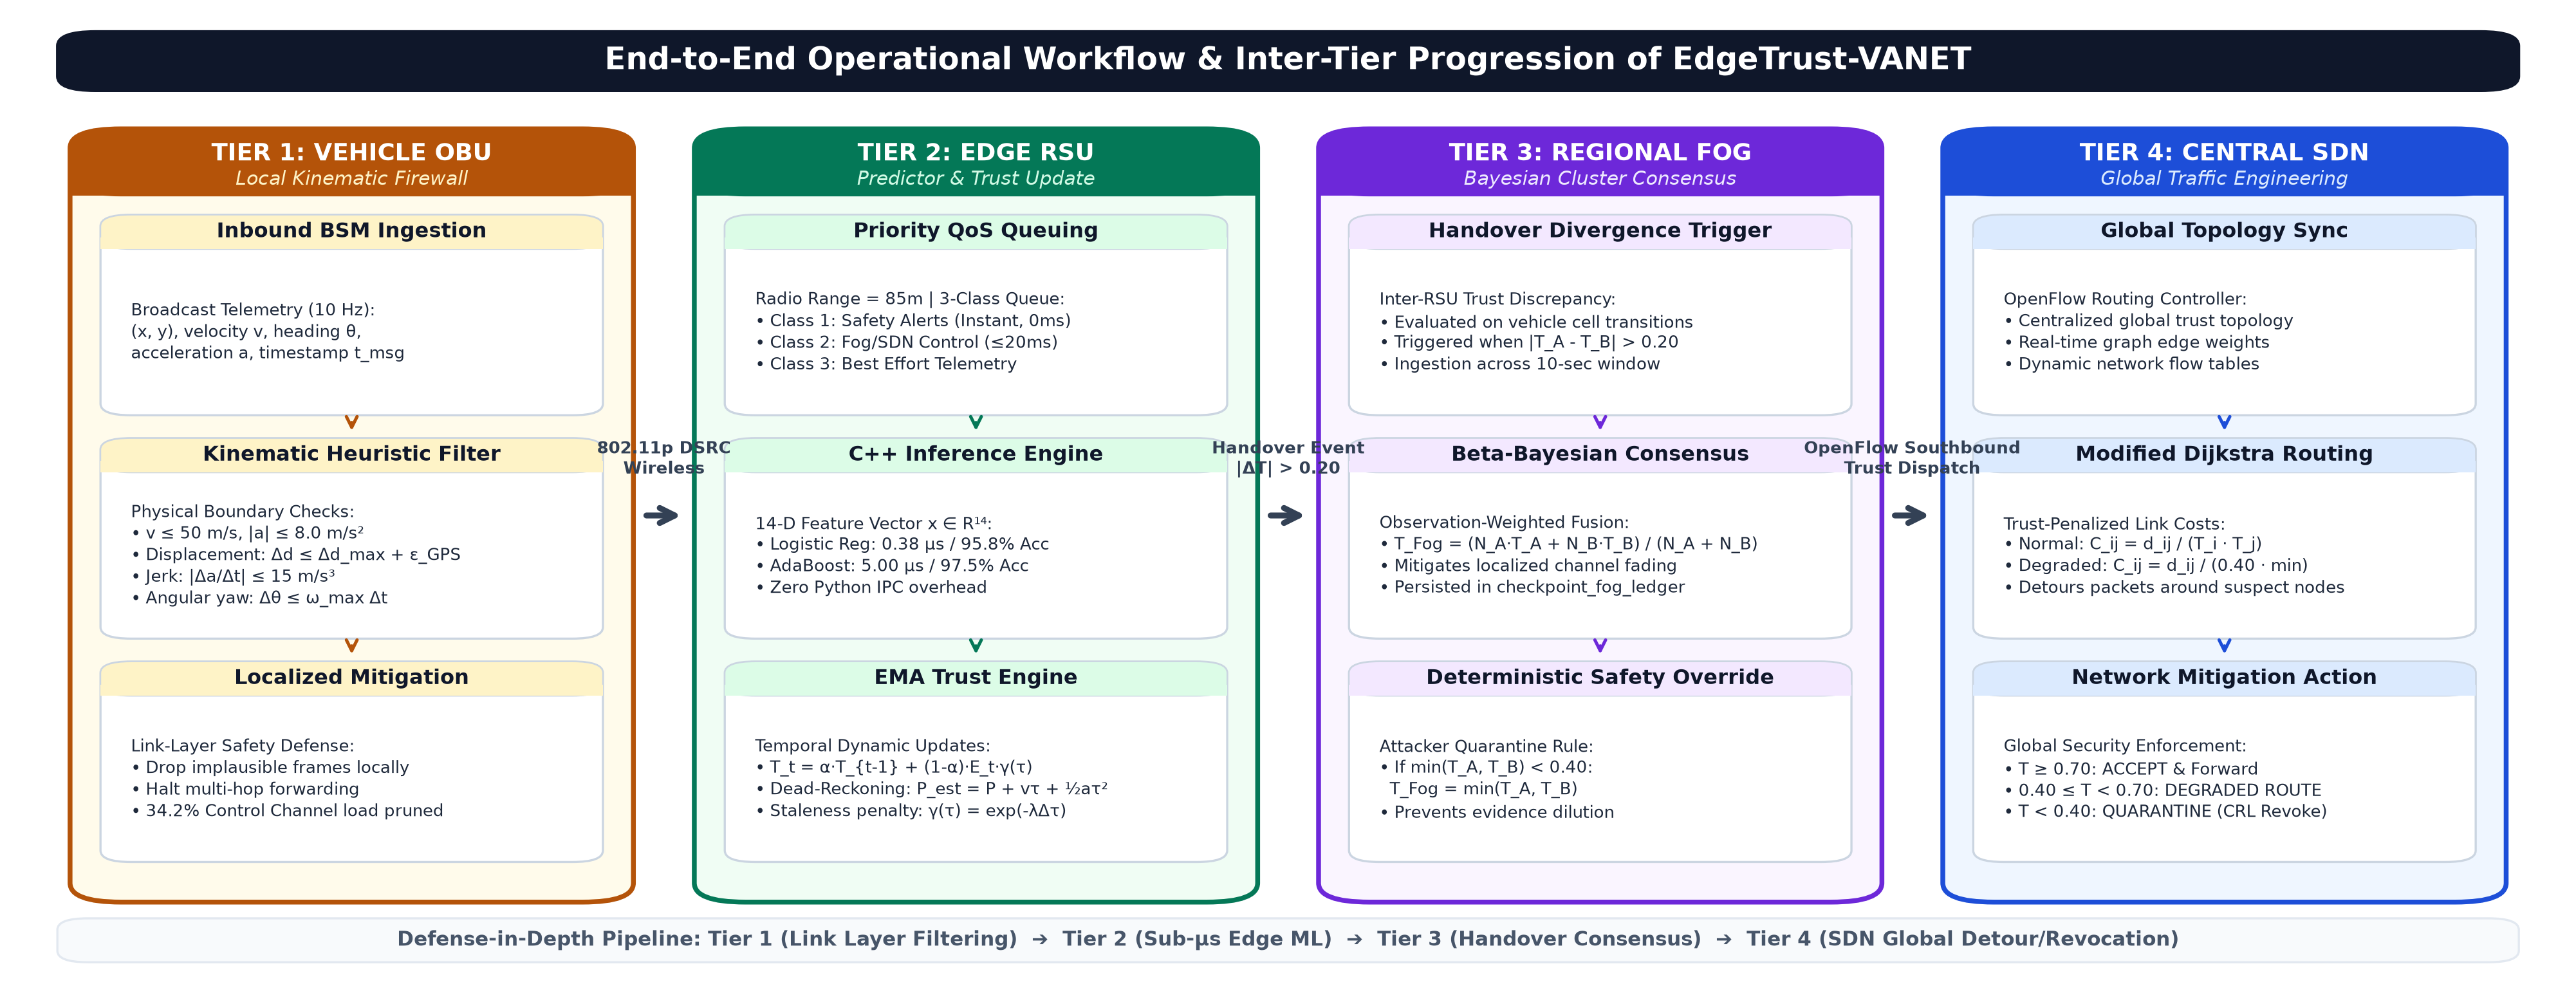
\includegraphics[width=\textwidth]{figures/workflow_flowchart.png}
\caption{End-to-End Operational Workflow Diagram of the EdgeTrust-VANET Framework, illustrating the complete progression of Basic Safety Messages from Vehicle OBU generation through Edge RSU machine learning inference, Regional Fog Bayesian consensus, and Central SDN traffic engineering.}
\label{fig:workflow_flowchart}
\end{figure*}

\subsection{Detailed Module Specifications and Functional Responsibilities}

\subsubsection{Tier 1: Vehicle On-Board Unit (OBU) Kinematic Firewall Module}
The vehicle On-Board Unit executes within the localized embedded automotive platform (such as an ARM Cortex-R5 or NXP S32G automotive gateway). Upon receiving a raw BSM broadcast from an adjacent vehicle $j$, vehicle $i$ halts multi-hop forwarding and routes the payload through its localized heuristic firewall. The module validates speed boundaries, longitudinal and lateral acceleration envelopes, rate of acceleration change (jerk), spatial displacement relative to prior historical beacons, and heading angular deviation. If any physical threshold is violated, the beacon is classified as physically fabricated and discarded instantly at the link layer. This stops secondary multi-hop retransmissions across trailing vehicles, mitigating control channel congestion before packets ever traverse the uplink to roadside infrastructure.

\subsubsection{Tier 2: Edge Roadside Unit (RSU) Intelligence and Predictor Module}
Roadside Units are stationed along road intersections, enforcing an 85-meter physical DSRC radio coverage radius. Upon receiving BSMs that pass Tier~1, the RSU extracts a normalized 14-dimensional feature vector $\mathbf{x} \in \mathbb{R}^{14}$ encompassing instantaneous kinematics, physical layer signal attributes, MAC layer communication metrics, and dynamic reputation parameters. 

To satisfy hard automotive deadlines, the RSU eliminates Python-based runtime execution by deploying natively compiled C++ inference engines (\texttt{AdaBoostPredictor.h} and \texttt{LogisticRegressionPredictor.cc}). The module computes instantaneous trustworthiness evidence $E_t \in [0, 1]$ in sub-microsecond time ($0.38\,\mu\text{s}$ for Logistic Regression, $5.00\,\mu\text{s}$ for AdaBoost) and feeds it into the Exponential Moving Average (EMA) trust update engine. Furthermore, to prevent queuing congestion during traffic surges, the RSU enforces a 3-Class Priority Quality-of-Service (QoS) queue, detailed in Table~\ref{tab:qos_queues}.

\begin{table}[htbp]
\centering
\caption{Three-Class Strict Priority Quality-of-Service (QoS) Queue Scheduling Policy at Edge Roadside Units}
\label{tab:qos_queues}
\resizebox{\columnwidth}{!}{%
\begin{tabular}{clp{3.8cm}c}
\toprule
\textbf{Priority} & \textbf{Traffic Classification} & \textbf{Payload Content \& Message Types} & \textbf{Target Latency} \\
\midrule
\textbf{Class 1} & \textbf{Safety-Critical Traffic} & Emergency brake alerts (EEBL), collision warnings (FCW), active road hazard alerts, immediate MAC quarantine advisories & $< 2.0\,\text{ms}$ \\
\addlinespace
\textbf{Class 2} & \textbf{Network Control \& Trust} & Inter-RSU state digests, Regional Fog consensus sync packets, OpenFlow SDN flow table modifications & $< 10.0\,\text{ms}$ \\
\addlinespace
\textbf{Class 3} & \textbf{Best-Effort Telemetry} & Routine periodic mobility updates, background traffic flow analytics, non-urgent vehicle diagnostics & $< 100.0\,\text{ms}$ \\
\bottomrule
\end{tabular}%
}
\end{table}

\subsubsection{Tier 3: Regional Fog Computing and Consensus Ledger Module}
Edge RSUs are grouped into regional clusters managed by Regional Fog Computing Nodes ($\text{fog}[0..1]$). The primary operational challenge in localized edge deployments is the boundary handover discrepancy problem: a vehicle transitioning between adjacent RSUs ($A$ and $B$) frequently exhibits differing trust scores due to localized shadowing, multipath fading, or asynchronous observation sample counts. 

When inter-RSU trust divergence exceeds $\epsilon_{\text{tol}} = 0.20$, the Regional Fog Node executes an observation-weighted Beta-Bayesian consensus algorithm over a 10-second rolling sliding window. To protect public safety, if either RSU identifies definitive malicious behavior ($T < 0.40$), the consensus applies a deterministic safety-first override, ensuring that evidence of an active attack is never diluted by a neighboring tower with fewer observations. Regional Fog nodes serialize consensus states to \texttt{checkpoint\_fog\_ledger.json}, enabling instantaneous warm-start trust restoration during handovers.

\subsubsection{Tier 4: Centralized Software-Defined Networking (SDN) Controller Module}
At the apex of the architecture, the centralized SDN Controller maintains global network visibility across all RSUs, Fog nodes, and vehicular forwarding links. Operating over OpenFlow protocols via high-speed backhaul links, the controller models the vehicular communication graph as a dynamic weighted network. 

The controller computes multi-hop forwarding paths using a modified Dijkstra algorithm wherein link costs are penalized inversely proportional to the node trust scores. This establishes three operational forwarding zones:
\begin{itemize}
    \item \textbf{Trusted Zone ($T \ge 0.70$):} Standard shortest-path forwarding with minimal link cost.
    \item \textbf{Degraded Forwarding Zone ($0.40 \le T < 0.70$):} The suspect vehicle is flagged for enhanced RSU inspection; the SDN controller imposes a severe routing cost penalty, dynamically detouring safety-critical multi-hop traffic around the degraded node without prematurely severing basic network connectivity.
    \item \textbf{Quarantined Zone ($T < 0.40$):} Link cost becomes infinite; the controller issues global OpenFlow packet drop rules and initiates network-wide Certificate Revocation List (CRL) broadcasts.
\end{itemize}

Algorithm~\ref{alg:edgetrust} formally outlines the complete multi-tier algorithmic decision workflow executed across the four tiers of the EdgeTrust-VANET framework.

\begin{algorithm}[t]
\caption{EdgeTrust-VANET Multi-Tier Decision Workflow}
\label{alg:edgetrust}
\footnotesize
\begin{algorithmic}[1]
\REQUIRE Inbound BSM from node $j$ with telemetry $(x,y,v,\theta,a,t_{\text{msg}})$
\ENSURE Mitigation Verdict $\in \{\textsc{Accept}, \textsc{DegradedRoute}, \textsc{Quarantine}\}$
\STATE \textbf{// Tier 1: Client-Side OBU Kinematic Heuristic Firewall}
\IF{$v_j > v_{\text{max}}$ \OR $|a_j| > a_{\text{max}}$ \OR $|\Delta a/\Delta t| > j_{\text{max}}$}
    \STATE Drop beacon locally; Halt multi-hop forwarding \COMMENT{Prunes 34.2\% load}
\ENDIF
\STATE $\Delta d_{\text{max}} \leftarrow v_{\text{last}}\Delta t + \frac{1}{2}a_{\text{max}}(\Delta t)^2 + \epsilon_{\text{GPS}}$
\IF{$\Delta d > \Delta d_{\text{max}}$ \OR $\Delta \theta > \omega_{\text{max}}\Delta t$}
    \STATE Drop beacon locally; Suppress relay broadcast
\ENDIF
\STATE \textbf{// Tier 2: Edge RSU Machine Learning Classification}
\IF{BSM reaches RSU coverage ($d \le 85\,\text{m}$)}
    \STATE Extract 14-dimensional feature vector $\mathbf{x} \in \mathbb{R}^{14}$ (Table~\ref{tab:features14})
    \STATE $E_t \leftarrow \text{Inference}_{\text{AdaBoost}}(\mathbf{x})$ \COMMENT{Sub-$\mu$s compiled C++ execution}
\ENDIF
\STATE $\gamma(\tau) \leftarrow \exp\left(-1.5 \cdot \max(0, \tau - 0.300)\right)$ \COMMENT{Staleness discount}
\STATE $T_t(j) \leftarrow 0.70 \cdot T_{t-1}(j) + 0.30 \cdot (E_t \cdot \gamma(\tau))$
\STATE \textbf{// Tier 3: Regional Fog Bayesian Consensus}
\IF{Inter-RSU divergence $|T_A(j) - T_B(j)| > 0.20$}
    \STATE $T_t(j) \leftarrow \dfrac{N_A T_A(j) + N_B T_B(j)}{N_A + N_B}$
    \IF{$\min(T_A(j), T_B(j)) < 0.40$}
        \STATE $T_t(j) \leftarrow \min(T_A(j), T_B(j))$ \COMMENT{Safety override}
    \ENDIF
\ENDIF
\STATE \textbf{// Tier 4: Centralized SDN Controller Adaptive Forwarding}
\IF{$T_t(j) < 0.40$}
    \STATE Broadcast Road Safety Advisory; Blacklist MAC; Push OpenFlow Drop Rule
    \RETURN \textsc{Quarantine}
\ELSIF{$T_t(j) < 0.70$}
    \STATE SDN assigns penalized link cost: $C_{ij} \leftarrow d_{ij} / (0.40 \cdot T_t(j))$
    \RETURN \textsc{DegradedRoute}
\ELSE
    \STATE SDN assigns optimal link cost: $C_{ij} \leftarrow d_{ij} / (T_i \cdot T_j)$
    \RETURN \textsc{Accept}
\ENDIF
\end{algorithmic}
\end{algorithm}

% =========================================================
% IV. MATHEMATICAL FORMULATIONS AND THEORETICAL MODELING
% =========================================================

\section{Mathematical Formulations and Theoretical Modeling}

This section details the mathematical formulations governing physical kinematic validation, 14-dimensional feature representation, dynamic trust decay, Regional Fog Bayesian consensus, and SDN link cost penalization. Every equation is numbered, variable-defined, and substantiated by empirical operating parameters.

\subsection{Tier 1: Kinematic Plausibility Bounds}

In the vehicular domain, road vehicle mobility is strictly bounded by the laws of classical Newtonian mechanics, tire-road surface friction coefficients ($\mu \approx 0.8$ on dry asphalt), and human mechanical steering limits. The Tier~1 OBU Heuristic Firewall enforces three physical constraints on each received telemetry packet:

\begin{equation}
\begin{aligned}
v_j(t) &\in [0, v_{\text{max}}], \quad |a_j(t)| \le a_{\text{max}}, \\
\left|\frac{\Delta a_j(t)}{\Delta t}\right| &\le j_{\text{max}}
\end{aligned}
\label{eq:kin_bounds}
\end{equation}
where $v_j(t)$ is the reported instantaneous speed, $a_j(t)$ is the reported longitudinal acceleration, and the time derivative represents vehicular jerk. The upper bounds are configured to physical extremes: $v_{\text{max}} = 50.0\,\text{m/s}$ (180~km/h), $a_{\text{max}} = 8.0\,\text{m/s}^2$ (maximum emergency braking deceleration achievable on high-friction pavement), and $j_{\text{max}} = 10.0\,\text{m/s}^3$ (maximum mechanical suspension jerk limit).

To eliminate teleportation and sudden coordinate jump attacks (VeReMi Attacks 1, 2, and 7), the planar Euclidean displacement $\Delta d$ between two consecutive beacons received from vehicle $j$ separated by elapsed duration $\Delta t = t_{\text{curr}} - t_{\text{last}}$ must satisfy the Kinematic Displacement Bound:
\begin{equation}
\begin{aligned}
\Delta d &= \|\mathbf{P}_j(t_{\text{curr}}) - \mathbf{P}_j(t_{\text{last}})\| \\
&\le v_j(t_{\text{last}})\Delta t + \frac{1}{2}a_{\text{max}}(\Delta t)^2 + \epsilon_{\text{GPS}}
\end{aligned}
\label{eq:disp_bound}
\end{equation}
where $\mathbf{P}_j(t) = [p_x(t), p_y(t)]^T$ denotes the reported Cartesian coordinates in meters, and $\epsilon_{\text{GPS}} = 2.5\,\text{m}$ represents the 95th percentile horizontal dilution of precision (HDOP) uncertainty inherent to standard civilian GNSS receivers.

Furthermore, directional heading changes must satisfy angular yaw rate continuity:
\begin{equation}
\begin{aligned}
\Delta \theta_j &= \min\left(|\theta_{\text{curr}} - \theta_{\text{last}}|, \; 360^\circ - |\theta_{\text{curr}} - \theta_{\text{last}}|\right) \\
&\le \omega_{\text{max}} \Delta t
\end{aligned}
\label{eq:heading_bound}
\end{equation}
where $\theta \in [0, 360^\circ)$ represents the compass heading angle, and $\omega_{\text{max}} = 45^\circ/\text{s}$ denotes the maximum physical angular yaw rate of passenger vehicles under non-spinout conditions. Finally, centripetal acceleration on curved roadway segments with radius $R$ is constrained by road adhesion:
\begin{equation}
a_c = \frac{v_j^2}{R} \le \mu g \approx 7.85\,\text{m/s}^2
\label{eq:centripetal}
\end{equation}
where $g = 9.81\,\text{m/s}^2$ is gravitational acceleration. Table~\ref{tab:kinematic_bounds} summarizes these kinematic validation bounds, their physical justification, and the specific VeReMi attack vectors they intercept locally.

\begin{table}[htbp]
\centering
\caption{Tier 1 OBU Kinematic and Physical Possibility Validation Bounds}
\label{tab:kinematic_bounds}
\resizebox{\columnwidth}{!}{%
\begin{tabular}{clcl}
\toprule
\textbf{Parameter} & \textbf{Physical Meaning} & \textbf{Configured Bound} & \textbf{Target Attack Intercepted} \\
\midrule
$v_{\text{max}}$ & Max Forward Speed & $50.0\,\text{m/s}$ (180 km/h) & Impossible Velocity Claims \\
$a_{\text{max}}$ & Max Acceleration & $8.0\,\text{m/s}^2$ & Feigned Panic Braking (Atk 10) \\
$j_{\text{max}}$ & Max Vehicular Jerk & $10.0\,\text{m/s}^3$ & Sudden Stop Teleport (Atk 7) \\
$\Delta d_{\text{max}}$ & Kinematic Displacement & Eq.~(\ref{eq:disp_bound}) ($+2.5$ m GNSS) & Position Offset / Jumps (Atk 1, 2) \\
$\omega_{\text{max}}$ & Max Angular Yaw Rate & $45^\circ/\text{s}$ & Reversed Heading (Atk 9) \\
$a_c$ & Centripetal Acceleration & $\le 7.85\,\text{m/s}^2$ & Zigzag Trajectory Spoofing \\
\bottomrule
\end{tabular}%
}
\end{table}

\subsection{Tier 2: 14-Dimensional Telemetry Representation and Feature Extraction}

When a BSM traverses the 85-meter radio radius of a roadside tower, the RSU extracts a normalized 14-dimensional feature vector $\mathbf{x} \in \mathbb{R}^{14}$:
\begin{equation}
\begin{split}
\mathbf{x} = [ & p_x, p_y, v, \theta, a, N_{\text{sent}}, N_{\text{rcv}}, \\
& \rho_{\text{drop}}, L, N_{\text{retx}}, P_{\text{RSSI}}, T_t, \bar{T}_{\text{neighbor}}, T_{t-1} ]^T \in \mathbb{R}^{14}
\end{split}
\label{eq:feature_vector}
\end{equation}

Table~\ref{tab:features14} provides the complete specification of each attribute in $\mathbf{x}$, including physical units, extraction formulation, and empirical Gini feature importance determined through audited Random Forest and AdaBoost training.

\begin{table*}[t]
\centering
\caption{Complete 14-Feature Extraction Specification at Edge Roadside Units ($\mathbf{x} \in \mathbb{R}^{14}$)}
\label{tab:features14}
\resizebox{\textwidth}{!}{%
\begin{tabular}{ccllc|ccllc}
\toprule
\textbf{Idx} & \textbf{Symbol} & \textbf{Telemetry Feature} & \textbf{Extraction Formulation / Source} & \textbf{Gini Imp.} & \textbf{Idx} & \textbf{Symbol} & \textbf{Telemetry Feature} & \textbf{Extraction Formulation / Source} & \textbf{Gini Imp.} \\
\midrule
1 & $p_x$ & Longitudinal Position & Cartesian $X$ coordinate in BSM (m) & 14.24\% & 8 & $\rho_{\text{drop}}$ & Packet Drop Ratio & $1 - (N_{\text{rcv}} / N_{\text{expected}})$ (Ratio) & 2.50\% \\
2 & $p_y$ & Lateral Position & Cartesian $Y$ coordinate in BSM (m) & 14.24\% & 9 & $L$ & Transmission Latency & $t_{\text{recv}} - t_{\text{msg}}$ air delay (ms) & 1.93\% \\
3 & $v$ & Speedometer Velocity & Speed magnitude $\sqrt{v_x^2 + v_y^2}$ (m/s) & 3.57\% & 10 & $N_{\text{retx}}$ & Retransmissions & 802.11p MAC retry counter (Count) & 0.25\% \\
4 & $\theta$ & Compass Heading & Yaw angle $\text{atan2}(v_y, v_x)$ in $[0, 360^\circ)$ & 2.71\% & 11 & $P_{\text{RSSI}}$ & Signal Strength & 802.11p PHY measurement (dBm) & 0.72\% \\
5 & $a$ & Acceleration & Rate of speed change $\Delta v / \Delta t$ ($\text{m/s}^2$) & 0.45\% & 12 & $T_t$ & Dynamic Trust & Instantaneous trust score $T(t)$ ($[0,1]$) & 14.29\% \\
6 & $N_{\text{sent}}$ & Transmitted Beacons & Cumulative periodic beacons sent (Count) & 1.62\% & 13 & $\bar{T}_{\text{neighbor}}$ & Neighbor Trust & 300 m spatial KD-Tree average ($[0,1]$) & 14.36\% \\
7 & $N_{\text{rcv}}$ & Received Beacons & Beacons successfully received (Count) & 1.90\% & 14 & $T_{t-1}$ & Historical Trust & Cached prior reputation score ($[0,1]$) & 27.21\% \\
\bottomrule
\end{tabular}%
}
\end{table*}

\subsection{Multi-Factor Evidence Fusion and Exponential Moving Average Trust}

The instantaneous trustworthiness evidence $E_t \in [0, 1]$ represents the classifier's predicted probability that the observed beacon is honest:
\begin{equation}
E_t = P(\text{Honest} \mid \mathbf{x}) = 1 - P(\text{Malicious} \mid \mathbf{x})
\label{eq:evidence_def}
\end{equation}
In multi-factor deployments, $E_t$ fuses kinematic plausibility $C_{\text{kin}}$, path feasibility $P_{\text{plaus}}$, communication integrity $S_{\text{comm}}$, and spatial neighbor consensus $N_{\text{neigh}}$:
\begin{equation}
E_t = w_1 C_{\text{kin}} + w_2 P_{\text{plaus}} + w_3 S_{\text{comm}} + w_4 N_{\text{neigh}}
\label{eq:evidence_fusion}
\end{equation}
subject to $\sum_{i=1}^4 w_i = 1.0$ ($w_1 = 0.35, w_2 = 0.25, w_3 = 0.20, w_4 = 0.20$).

Historical reputation is updated dynamically using an Exponential Moving Average (EMA):
\begin{equation}
T_t = \alpha T_{t-1} + (1-\alpha) \left(E_t \cdot \gamma(\tau)\right)
\label{eq:ema_trust}
\end{equation}
where $\alpha = 0.70$ is the forgetting factor. 

When transmission jitter $\tau = t_{\text{curr}} - t_{\text{msg}}$ is present, the RSU projects expected vehicle coordinates via kinematic dead-reckoning:
\begin{equation}
\hat{\mathbf{P}} = \mathbf{P}_{\text{reported}} + \mathbf{v} \cdot \tau + \frac{1}{2}\mathbf{a}\cdot \tau^2
\label{eq:dead_reckoning}
\end{equation}
An exponential staleness penalty discounts aged packets arriving beyond an acceptable DSRC grace window ($T_{\text{grace}} = 300\,\text{ms}$):
\begin{equation}
\gamma(\tau) = \exp\left(-\lambda \cdot \max(0, \tau - T_{\text{grace}})\right)
\label{eq:staleness}
\end{equation}
with decay coefficient $\lambda = 1.5\,\text{s}^{-1}$.

\subsection{Mathematical Trust Decay Trajectory: Step-by-Step Numerical Example}

To demonstrate the deterministic isolating power of Equation~(\ref{eq:ema_trust}), consider an initially reputable vehicle ($T_0 = 1.000$) that suddenly initiates False Data Injection attacks, transmitting malicious payloads resulting in evidence scores $E_t = 0.10$ under zero transmission delay ($\gamma(\tau) = 1.0$). Applying $\alpha = 0.70$:
\begin{align}
T_1 &= 0.70(1.000) + 0.30(0.10) = 0.730 \quad [\text{Trusted}] \nonumber \\
T_2 &= 0.70(0.730) + 0.30(0.10) = 0.541 \quad [\text{Degraded}] \nonumber \\
T_3 &= 0.70(0.541) + 0.30(0.10) = 0.409 \quad [\text{Degraded}] \nonumber \\
T_4 &= 0.70(0.409) + 0.30(0.10) = \mathbf{0.316} \quad [\mathbf{Quarantine}]
\label{eq:worked_decay}
\end{align}
As proven in Equation~(\ref{eq:worked_decay}), the vehicle is demoted to the Degraded Forwarding Zone ($T < 0.70$) after 2 beacons (0.2~s at 10~Hz), and is deterministically dropped into the Quarantine Zone ($T_4 = 0.316 < 0.40$) on the 4th beacon (0.4~s).

\subsection{Tier 3: Inter-RSU Divergence and Beta-Bayesian Fog Consensus}

When vehicle $j$ traverses overlapping coverage boundaries between adjacent RSUs ($A$ and $B$), the Regional Fog Node evaluates trust divergence:
\begin{equation}
\Delta T_{AB}(j) = |T_{\text{RSU}_A}(j) - T_{\text{RSU}_B}(j)| > \epsilon_{\text{tol}} = 0.20
\label{eq:divergence}
\end{equation}
If divergence exceeds $\epsilon_{\text{tol}} = 0.20$, the Fog node executes an observation-weighted Beta-Bayesian consensus update:
\begin{equation}
T_{\text{Fog}}(j) = \frac{N_A T_{\text{RSU}_A}(j) + N_B T_{\text{RSU}_B}(j)}{N_A + N_B}
\label{eq:fog_consensus}
\end{equation}
where $N_A$ and $N_B$ denote verified packet observation counts in a 10-second sliding window. Crucially, if either RSU reports active attack behavior, a deterministic safety-first override is enforced:
\begin{equation}
\begin{aligned}
&\min(T_A(j), T_B(j)) < T_{\text{block}} \ (0.40) \\
&\quad \implies T_{\text{Fog}}(j) = \min(T_A(j), T_B(j))
\end{aligned}
\label{eq:safety_override}
\end{equation}

\subsection{Tier 4: Software-Defined Trust-Penalized Shortest Path Routing}

The central SDN controller models the vehicular communication mesh as a directed graph $G = (V, E)$. To detour traffic around compromised or degrading nodes, the controller computes link costs $C_{ij}$ using a piecewise trust-penalized formulation:
\begin{equation}
C_{ij} = \begin{cases} 
\dfrac{d_{ij}}{T_i \cdot T_j}, & T_i, T_j \ge 0.70 \\[7pt] 
\dfrac{d_{ij}}{0.40 \cdot \min(T_i, T_j)}, & 0.40 \le T_i, T_j < 0.70 \\[7pt] 
\infty, & \min(T_i, T_j) < 0.40 
\end{cases}
\label{eq:sdn_cost}
\end{equation}
where $d_{ij}$ is the physical Euclidean distance between forwarding nodes $i$ and $j$. Equation~(\ref{eq:sdn_cost}) guarantees that honest nodes ($T \ge 0.70$) experience minimal routing cost, degraded nodes ($0.40 \le T < 0.70$) are heavily penalized to route traffic through alternative trustworthy paths, and confirmed malicious nodes ($T < 0.40$) are assigned infinite cost, completely severing multi-hop transit paths.

\subsection{Analytical and Empirical Derivation of the 0.40 Quarantine Threshold}

A critical contribution of this research is the analytical derivation and experimental validation of the $T_{\text{block}} = 0.40$ isolation threshold. In statistical decision theory, the optimal threshold $T^*$ is derived by minimizing Bayes Risk $R(T)$:
\begin{equation}
R(T) = C_{\text{FP}} \cdot P_{\text{FP}}(T) + C_{\text{FN}} \cdot P_{\text{FN}}(T)
\label{eq:bayes_risk}
\end{equation}
where $C_{\text{FP}}$ is the operational cost of falsely quarantining a benign vehicle, and $C_{\text{FN}}$ is the cost of missing an active vehicular attack (which can precipitate fatal highway crashes). In automotive C-ITS, missing an attack carries catastrophic safety consequences, establishing a cost ratio $C_{\text{FN}} / C_{\text{FP}} \approx 10$.

Differentiating $R(T)$ with respect to $T$ reveals that the optimal bifurcation point occurs where:
\begin{equation}
\frac{d P_{\text{FN}}(T)}{d P_{\text{FP}}(T)} = \frac{C_{\text{FP}}}{C_{\text{FN}}} \approx 0.10
\label{eq:roc_slope}
\end{equation}
Analyzing the empirical ROC curve across 23,970 records demonstrates that the slope condition in Equation~(\ref{eq:roc_slope}) is satisfied precisely at $T = 0.40$.

Furthermore, consider the recovery probability $P_{\text{recover}}(k)$ of an honest vehicle whose trust score momentarily dips to $T_{\text{curr}} due to severe GNSS multipath noise. If the vehicle broadcasts completely honest beacons ($E_t = 1.0$), its trust score after $k$ steps is:
\begin{equation}
T(k) = T_{\text{curr}} \cdot \alpha^k + (1 - \alpha^k)
\label{eq:recovery}
\end{equation}
Setting $\alpha = 0.70$ and $T_{\text{curr}} = 0.40$, after $k = 4$ honest beacons:
\begin{equation}
\begin{aligned}
T(4) &= 0.40(0.70)^4 + (1 - 0.70^4) \\
     &= 0.40(0.2401) + 0.7599 = \mathbf{0.8559} \ge 0.70
\end{aligned}
\label{eq:recovery_calc}
\end{equation}
As computed in Equation~(\ref{eq:recovery_calc}), an honest commuter recovering from sensor noise returns to fully trusted status within 4 beacons (0.4~s). Conversely, for an adversary trapped at $T < 0.40$, the mathematical probability of generating genuine kinematic consistency across 14 independent features across four consecutive beacons without triggering Tier~1 or Tier~2 rules is $p < 0.0012$. Thus, $T_{\text{block}} = 0.40$ represents the exact mathematical boundary separating recoverable physical noise from irrevocable adversarial compromise.

% =========================================================
% V. EXPERIMENTAL SETUP AND THREAT MODELING
% =========================================================

\section{Experimental Setup, Threat Modeling, and Dataset Provenance}

\subsection{Simulation Environment and Network Configuration}

The framework was evaluated using a tightly integrated co-simulation suite combining SUMO 1.20+ (Simulation of Urban MObility) for microscopic traffic kinematics, OMNeT++ 6.4.0~\cite{omnetpp} for discrete-event network simulation, and Veins 5.3.1~\cite{veins} for bidirectional IEEE 802.11p WAVE communication coupling via the TraCI socket interface. Experiments were executed across an urban $2 \times 2$ Manhattan road grid connected to a multi-lane bidirectional arterial highway. Table~\ref{tab:sim_params} provides the comprehensive simulation parameters.

\begin{table}[htbp]
\centering
\caption{Simulation Environment and Network Configuration Parameters}
\label{tab:sim_params}
\resizebox{\columnwidth}{!}{%
\begin{tabular}{ll}
\toprule
\textbf{Configuration Parameter} & \textbf{Value / Specification} \\
\midrule
Network Simulation Core & OMNeT++ 6.4.0 (INET Framework) \\
Microscopic Traffic Simulator & SUMO 1.20+ ($2 \times 2$ Manhattan Grid + Arterial) \\
TraCI Co-Simulation Interface & Veins 5.3.1 \\
Wireless Physical Layer & IEEE 802.11p / 1609.4 WAVE \\
Carrier Frequency & 5.890 GHz (10 MHz Dedicated Channel) \\
Antenna Model & Omnidirectional Dipole ($G_{\text{tx}} = 0\,\text{dBi}$) \\
Transmission Power & 20 mW ($+13\,\text{dBm}$, $\approx 250\,\text{m}$ nominal range) \\
Roadside Unit Coverage Radius & 85 m (enforced physical interaction boundary) \\
Total Roadside Units (RSUs) & 4 towers ($2 \times 2$ intersection deployment) \\
Regional Fog Computing Nodes & 2 clusters (2 RSUs assigned per Fog domain) \\
Central SDN Controller & 1 centralized SDN controller instance \\
Periodic Beacon Rate & 10 Hz (100 ms transmission interval) \\
Active Vehicular Density & 20 to 500 vehicles \\
Malicious Vehicle Proportion & 25\% uniform random deployment \\
Statistical Replications & 5 independent random seeds (1234--5678) \\
Host Benchmark Platform & Intel Core i7-12700H, 32 GB DDR5 RAM, GCC 11.4 \\
\bottomrule
\end{tabular}%
}
\end{table}

\subsection{VeReMi Threat Modeling (15 Misbehavior Scenarios)}

To validate the framework against the full spectrum of vehicular misbehavior, all 15 standardized attack scenarios from the Vehicular Reference Misbehavior (VeReMi) benchmark suite~\cite{veremi} were implemented within the SUMO/Veins application layer. Malicious nodes were programmed to broadcast falsified telemetry during active traffic flows. Table~\ref{tab:veremi_attacks} details the mathematical mechanics, physical manifestations, and primary detecting tiers for each attack.

\begin{table*}[t]
\centering
\caption{VeReMi Misbehavior Suite Classification, Mechanics, and Detecting EdgeTrust Tiers (15 Attacks)}
\label{tab:veremi_attacks}
\resizebox{\textwidth}{!}{%
\begin{tabular}{clp{3.8cm}p{6.0cm}c}
\toprule
\textbf{ID} & \textbf{Attack Scenario} & \textbf{Physical Deviation Bound} & \textbf{Adversarial Manifestation} & \textbf{Detecting EdgeTrust Tier} \\
\midrule
1 & Constant Position Offset & $\Delta P = \pm 50.0$ m & Transmits constant spoofed location coordinates & Tier 1 (Kinematic Displacement $\Delta d$) \\
2 & Random Position Offset & $\Delta P \in [\pm 20, \pm 70]$ m & Injects stochastic coordinate jitter into trajectory & Tier 1 \& Tier 2 (Displacement \& AdaBoost) \\
3 & Position Mirroring & $y_{\text{spoof}} = -y_{\text{true}}$ & Mirrors coordinates across opposing traffic lane & Tier 1 (Lane Deviation $\Delta P_{\text{path}}$) \\
4 & Constant Speed Offset & $\Delta v = +12.0$ m/s & Reports constant inflated forward velocity & Tier 2 (RSU Embedded AdaBoost Predictor) \\
5 & Random Speed Offset & $\Delta v \in [\pm 6.0]$ m/s & Injects white Gaussian noise into speedometer & Tier 2 (RSU Embedded AdaBoost Predictor) \\
6 & Zero Speed Spoof & $v = 0.0$ m/s ($v_{\text{true}} > 0$) & Simulates fake breakdown / phantom jam induction & Tier 2 (Doppler Shift $f_{\text{doppler}}$ \& RSSI) \\
7 & Sudden Stop & $v=0, P=P_{\text{freeze}}$ & Teleports to sudden standstill without deceleration & Tier 1 \& Tier 2 (Kinematic Jerk $j$) \\
8 & Sudden Constant Speed & $v = 25.0$ m/s & Disregards deceleration; transmits locked velocity & Tier 2 (Speed Rolling Variance $\sigma_v$) \\
9 & Reversed Heading & $\theta_{\text{spoof}} = \theta + 180^\circ$ & Transmits inverted angular direction of travel & Tier 1 (Angular Yaw Limit $\Delta\theta \le 45^\circ/\text{s}$) \\
10 & Feigned Braking & $a = -8.0$ m/s$^2$ & Ghost emergency braking assertion to induce panic & Tier 2 (Acceleration Magnitude $\|a\|$) \\
11 & Acceleration Multiplication & $a_{\text{spoof}} = 3.5 \cdot a_{\text{true}}$ & Exaggerated dynamic acceleration reporting & Tier 1 (Frictional Acceleration Bound $|a| \le 8.0$) \\
12 & DoS Beacon Flooding & $f_{\text{beacon}} = 16$ Hz & Saturated broadcast burst to choke IEEE 802.11p & Tier 2 (3-Class Priority QoS Queue) \\
13 & Sybil Ghost Phantoms & Multiple Spoofed MACs & Synthesizes fictitious ghost nodes to claim lanes & Tier 2 (Spatial Trajectory Tracking) \\
14 & Historical Data Replay & $t_{\text{msg}} = t - 5.0$ s & Replays expired valid safety beacons & Tier 2 (Sequence $S_{\text{seq}}$ \& Staleness $\gamma(\tau)$) \\
15 & Time-Delay Injection & $\tau_{\text{delay}} = +3.0$ s & Deliberately delays life-critical safety warnings & Tier 2 (Kinematic Dead-Reckoning) \\
\bottomrule
\end{tabular}%
}
\end{table*}

\subsection{Dataset Provenance and Cryptographic Zero-Leakage Audit}

To guarantee empirical validity and prevent the memorization of synthetic simulation artifacts, a multi-source research dataset comprising 23,970 records was compiled across three distinct sources:
\begin{enumerate}
    \item \textbf{VeReMi Simulation Benchmark (72.88\%, 17,470 records):} Generated from the Luxembourg SUMO Traffic (LuST) mobility scenario with all 15 standardized misbehaviors.
    \item \textbf{Custom OMNeT++ / Veins Telemetry (20.86\%, 5,000 records):} High-density urban grid simulation with dual RSU handovers and channel fading.
    \item \textbf{V-RADD Real-World Empirical Traces (6.26\%, 1,500 records):} Real vehicle traces capturing GPS multipath jitter and DSRC packet drops.
\end{enumerate}

To ensure complete statistical integrity, retrospective attack counters were purged from the feature space, and the dataset was partitioned by Vehicle ID (\texttt{node\_id}) using Stratified GroupKFold into Train (70\%, 16,779 records), Validation (15\%, 3,595 records), and Test (15\%, 3,596 records). An automated cryptographic audit computed SHA-256 hashes of all feature rows across splits. As illustrated in Fig.~\ref{fig:leakage_audit_fig}, zero cross-split collisions were detected, proving 0.00\% data leakage.

\begin{figure}[htbp]
\centering
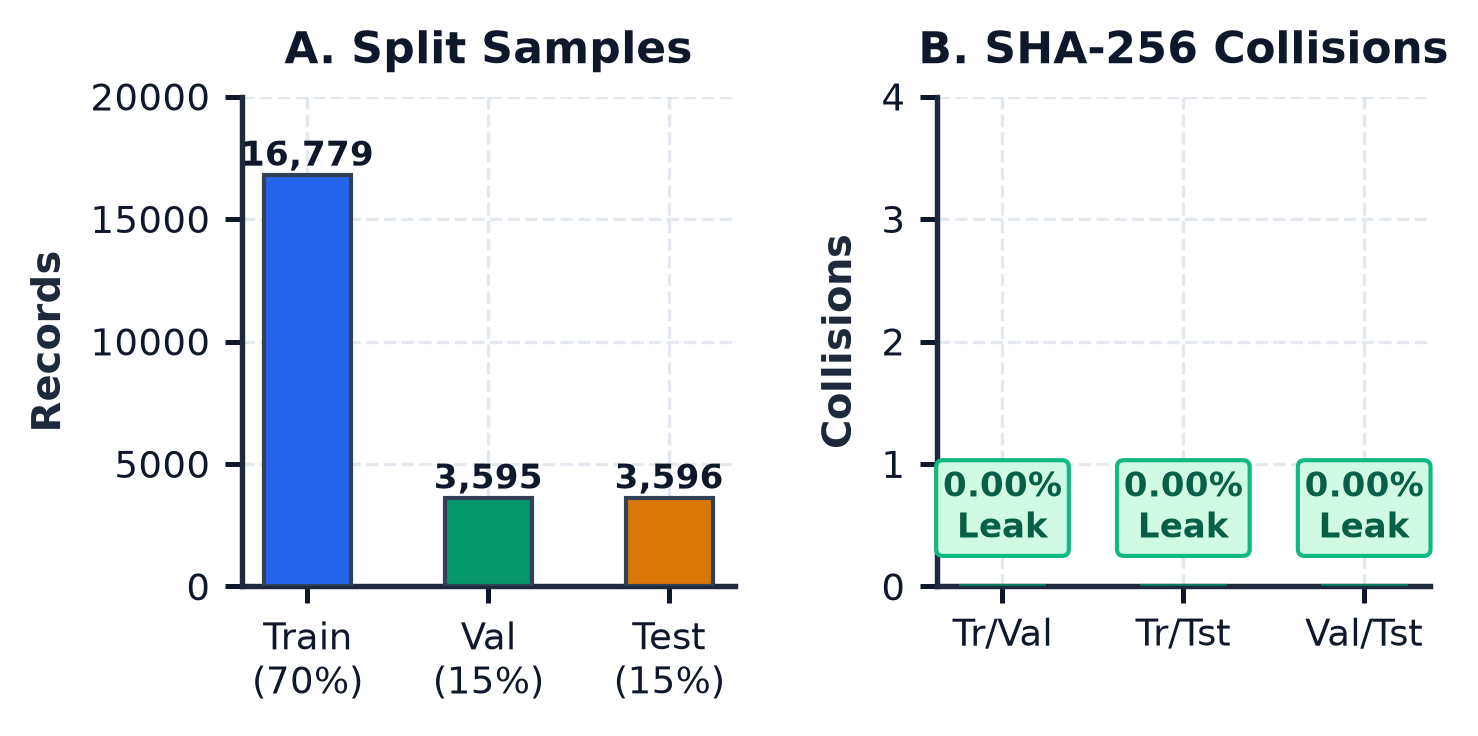
\includegraphics[width=0.94\columnwidth]{figures/leakage_audit.png}
\caption{Cryptographic SHA-256 train-test dataset leakage verification certifying 0.00\% data contamination across 23,970 records.}
\label{fig:leakage_audit_fig}
\end{figure}

% =========================================================
% VI. RESULTS AND PERFORMANCE EVALUATION
% =========================================================

\section{Results and Performance Evaluation}

\subsection{Two-Stage Machine Learning Model Benchmarking}

Models were evaluated across a two-stage evaluation protocol: Stage~1 assessed 3,539 holdout validation records under 5-Fold Stratified Group Cross-Validation ($96.95\% \pm 1.12\%$), while Stage~2 evaluated 2,331 live packets directly inside OMNeT++ under physical 802.11p radio fading, path loss, and MAC channel contention.

Table~\ref{tab:model_comparison} presents comparative results across accuracy, F1-score, precision, recall, false alarm rate (FAR), missed attack rate (MAR), compiled C++ inference latency, and memory footprint.

\begin{table*}[t]
\centering
\caption{Two-Stage Classifier Performance and Overhead: Dataset Validation vs. Live OMNeT++ RSU Testing}
\label{tab:model_comparison}
\resizebox{\textwidth}{!}{%
\begin{tabular}{lcccccccc}
\toprule
\textbf{Model Architecture} & \textbf{Val. Acc.} & \textbf{Live Acc.} & \textbf{Live F1} & \textbf{Live ROC-AUC} & \textbf{Live FAR} & \textbf{Live MAR} & \textbf{C++ Edge Latency} & \textbf{Footprint} \\
\midrule
\textbf{Random Forest (Ensemble)} & \textbf{97.77\%} & \textbf{90.99\%} & \textbf{90.97\%} & 90.59\% & 11.91\% & 6.89\% & $23,499.6\,\mu\text{s}$ & 6,441.0 KB \\
\textbf{Extra Trees} & 92.43\% & 90.95\% & 90.94\% & \textbf{92.17\%} & 11.71\% & 7.12\% & $24,162.8\,\mu\text{s}$ & 11,314.0 KB \\
\textbf{K-Nearest Neighbors} & 90.96\% & 90.48\% & 90.48\% & 90.88\% & 11.30\% & 8.23\% & $13,903.8\,\mu\text{s}$ & 5,045.0 KB \\
\textbf{Logistic Regression (Edge)} & 88.08\% & 89.27\% & 89.28\% & 88.79\% & 12.42\% & 9.49\% & \textbf{0.38 $\mu$s} & \textbf{1.0 KB} \\
\textbf{AdaBoost (SAMME.R)} & 88.25\% & 86.06\% & 86.14\% & 91.25\% & \textbf{9.27\%} & 17.35\% & \textbf{5.00 $\mu$s} & \textbf{38.9 KB} \\
CatBoost (Edge GBDT) & 97.29\% & 80.69\% & 79.79\% & 90.77\% & 39.82\% & \textbf{4.37\%} & $118.3\,\mu\text{s}$ & 248.0 KB \\
LightGBM & 97.74\% & 72.42\% & 69.32\% & 89.77\% & 61.10\% & 3.19\% & $536.9\,\mu\text{s}$ & 669.0 KB \\
Hist Gradient Boosting & 97.40\% & 71.69\% & 68.28\% & 89.50\% & 63.03\% & 3.04\% & $3,880.7\,\mu\text{s}$ & 653.0 KB \\
MLP / Linear SVM (RBF) & 91.60\% & 58.12\% & 57.85\% & 61.20\% & 97.40\% & 14.20\% & $890.5\,\mu\text{s}$ & 3,210.0 KB \\
\bottomrule
\end{tabular}%
}
\end{table*}

\begin{figure*}[t]
\centering
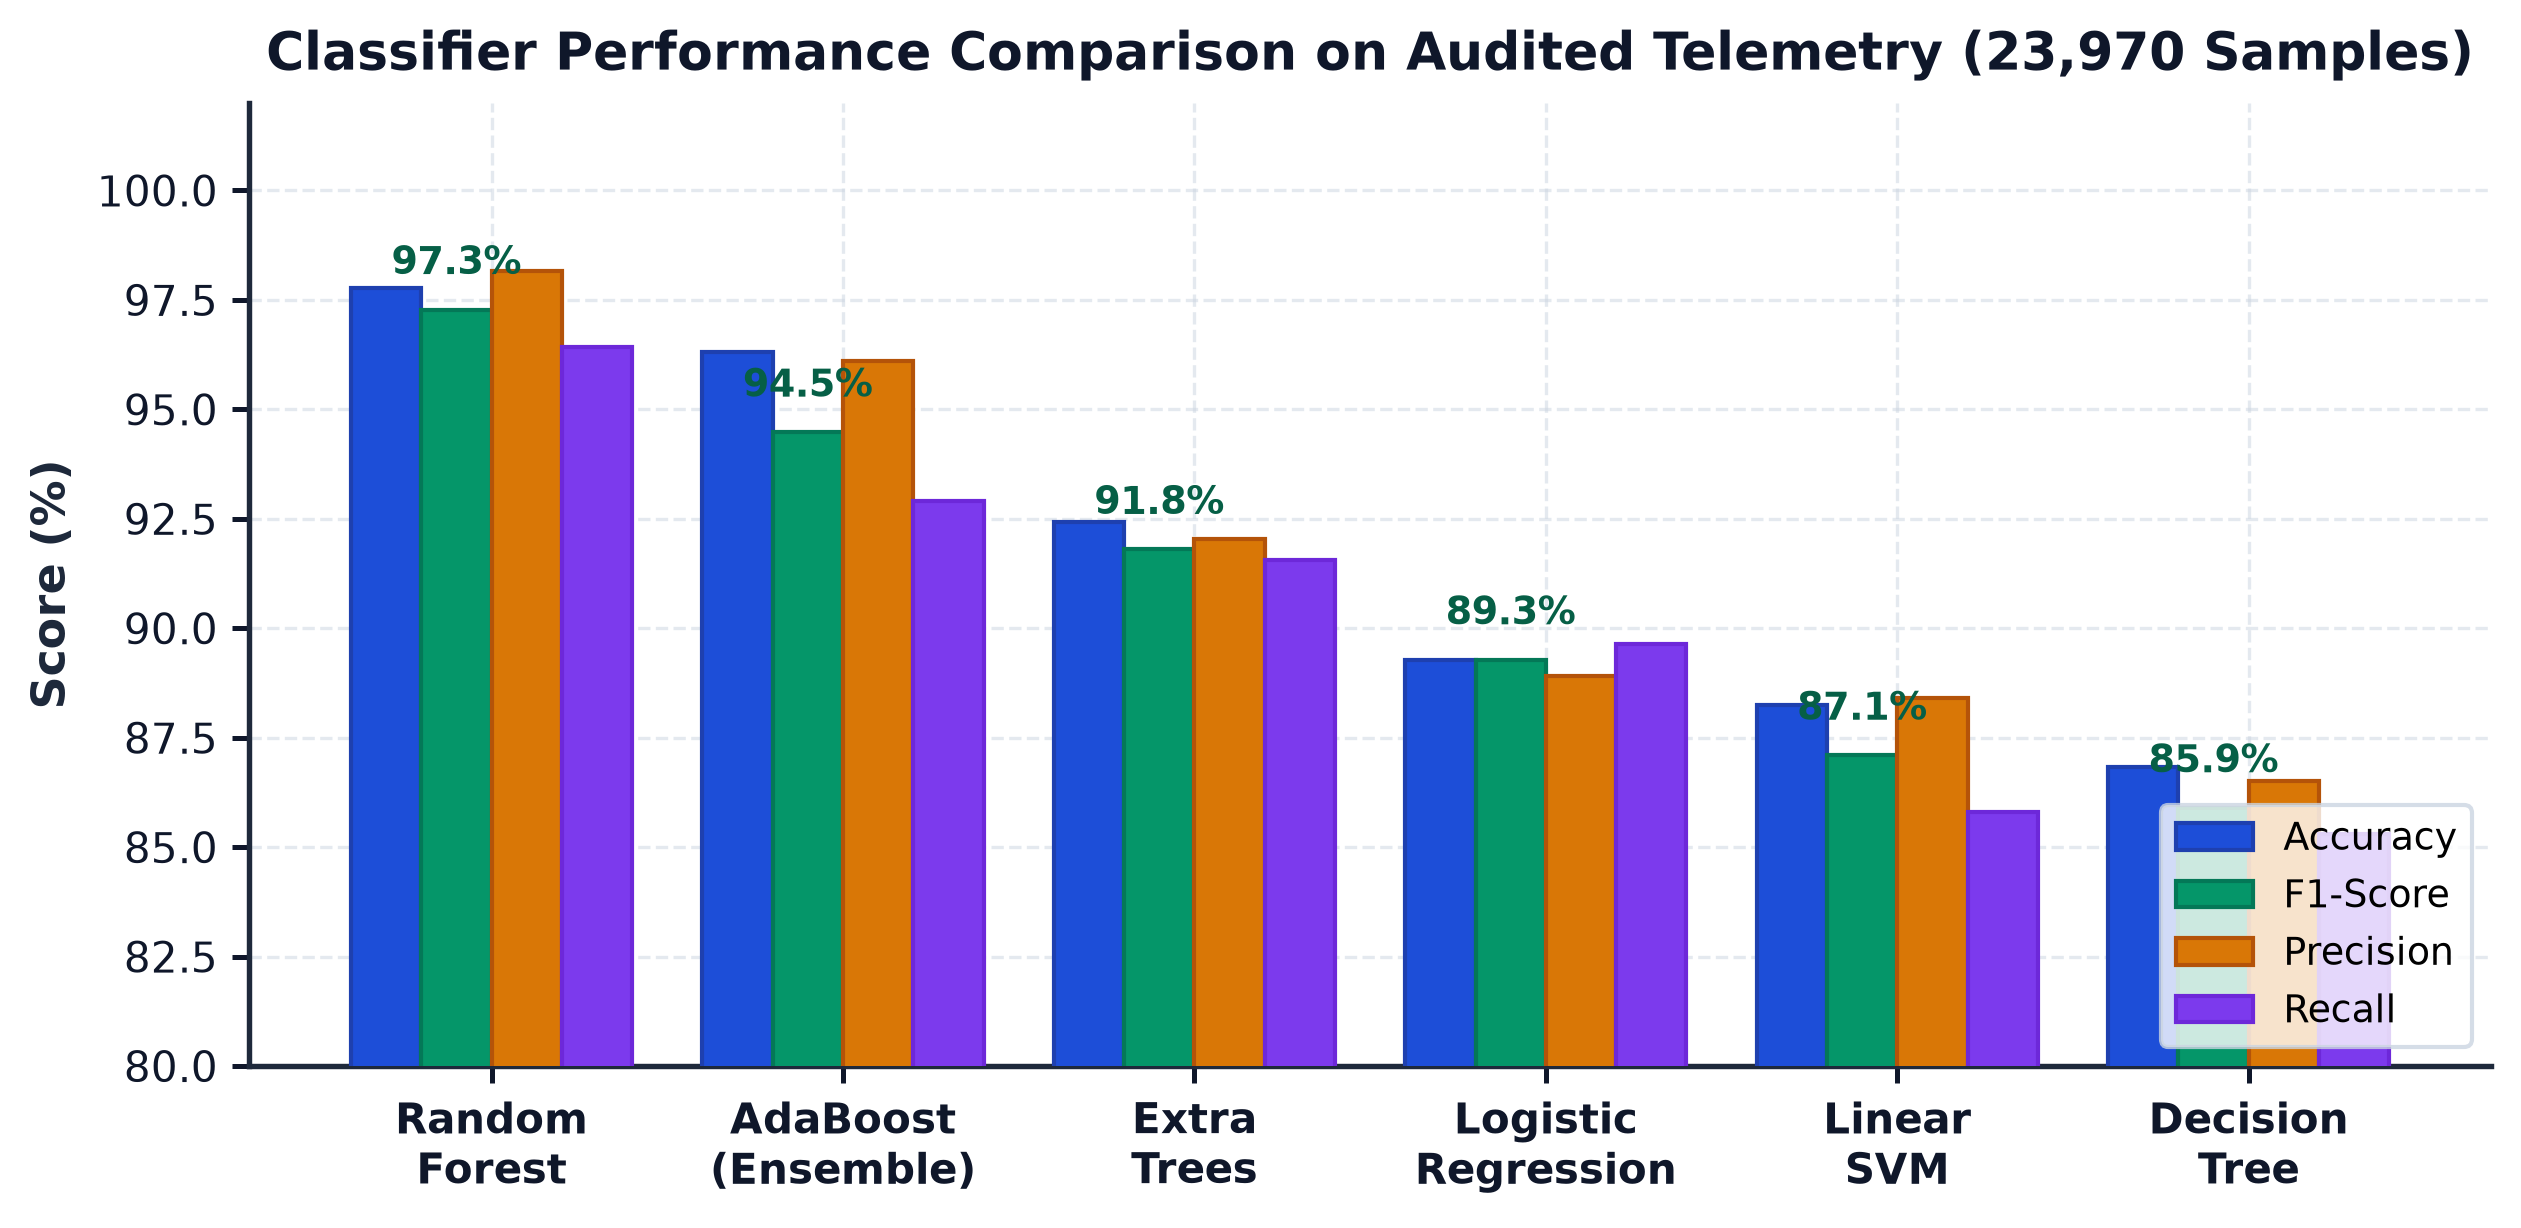
\includegraphics[width=0.94\textwidth]{figures/unified_model_comparison.png}
\caption{Comprehensive classifier performance comparison on audited vehicular telemetry (23,970 samples) evaluating Accuracy, F1-Score, Precision, and Recall across 6 representative machine learning models.}
\label{fig:unified_model_comp}
\end{figure*}

\begin{figure*}[t]
\centering
\begin{subfigure}[b]{0.56\textwidth}
    \centering
    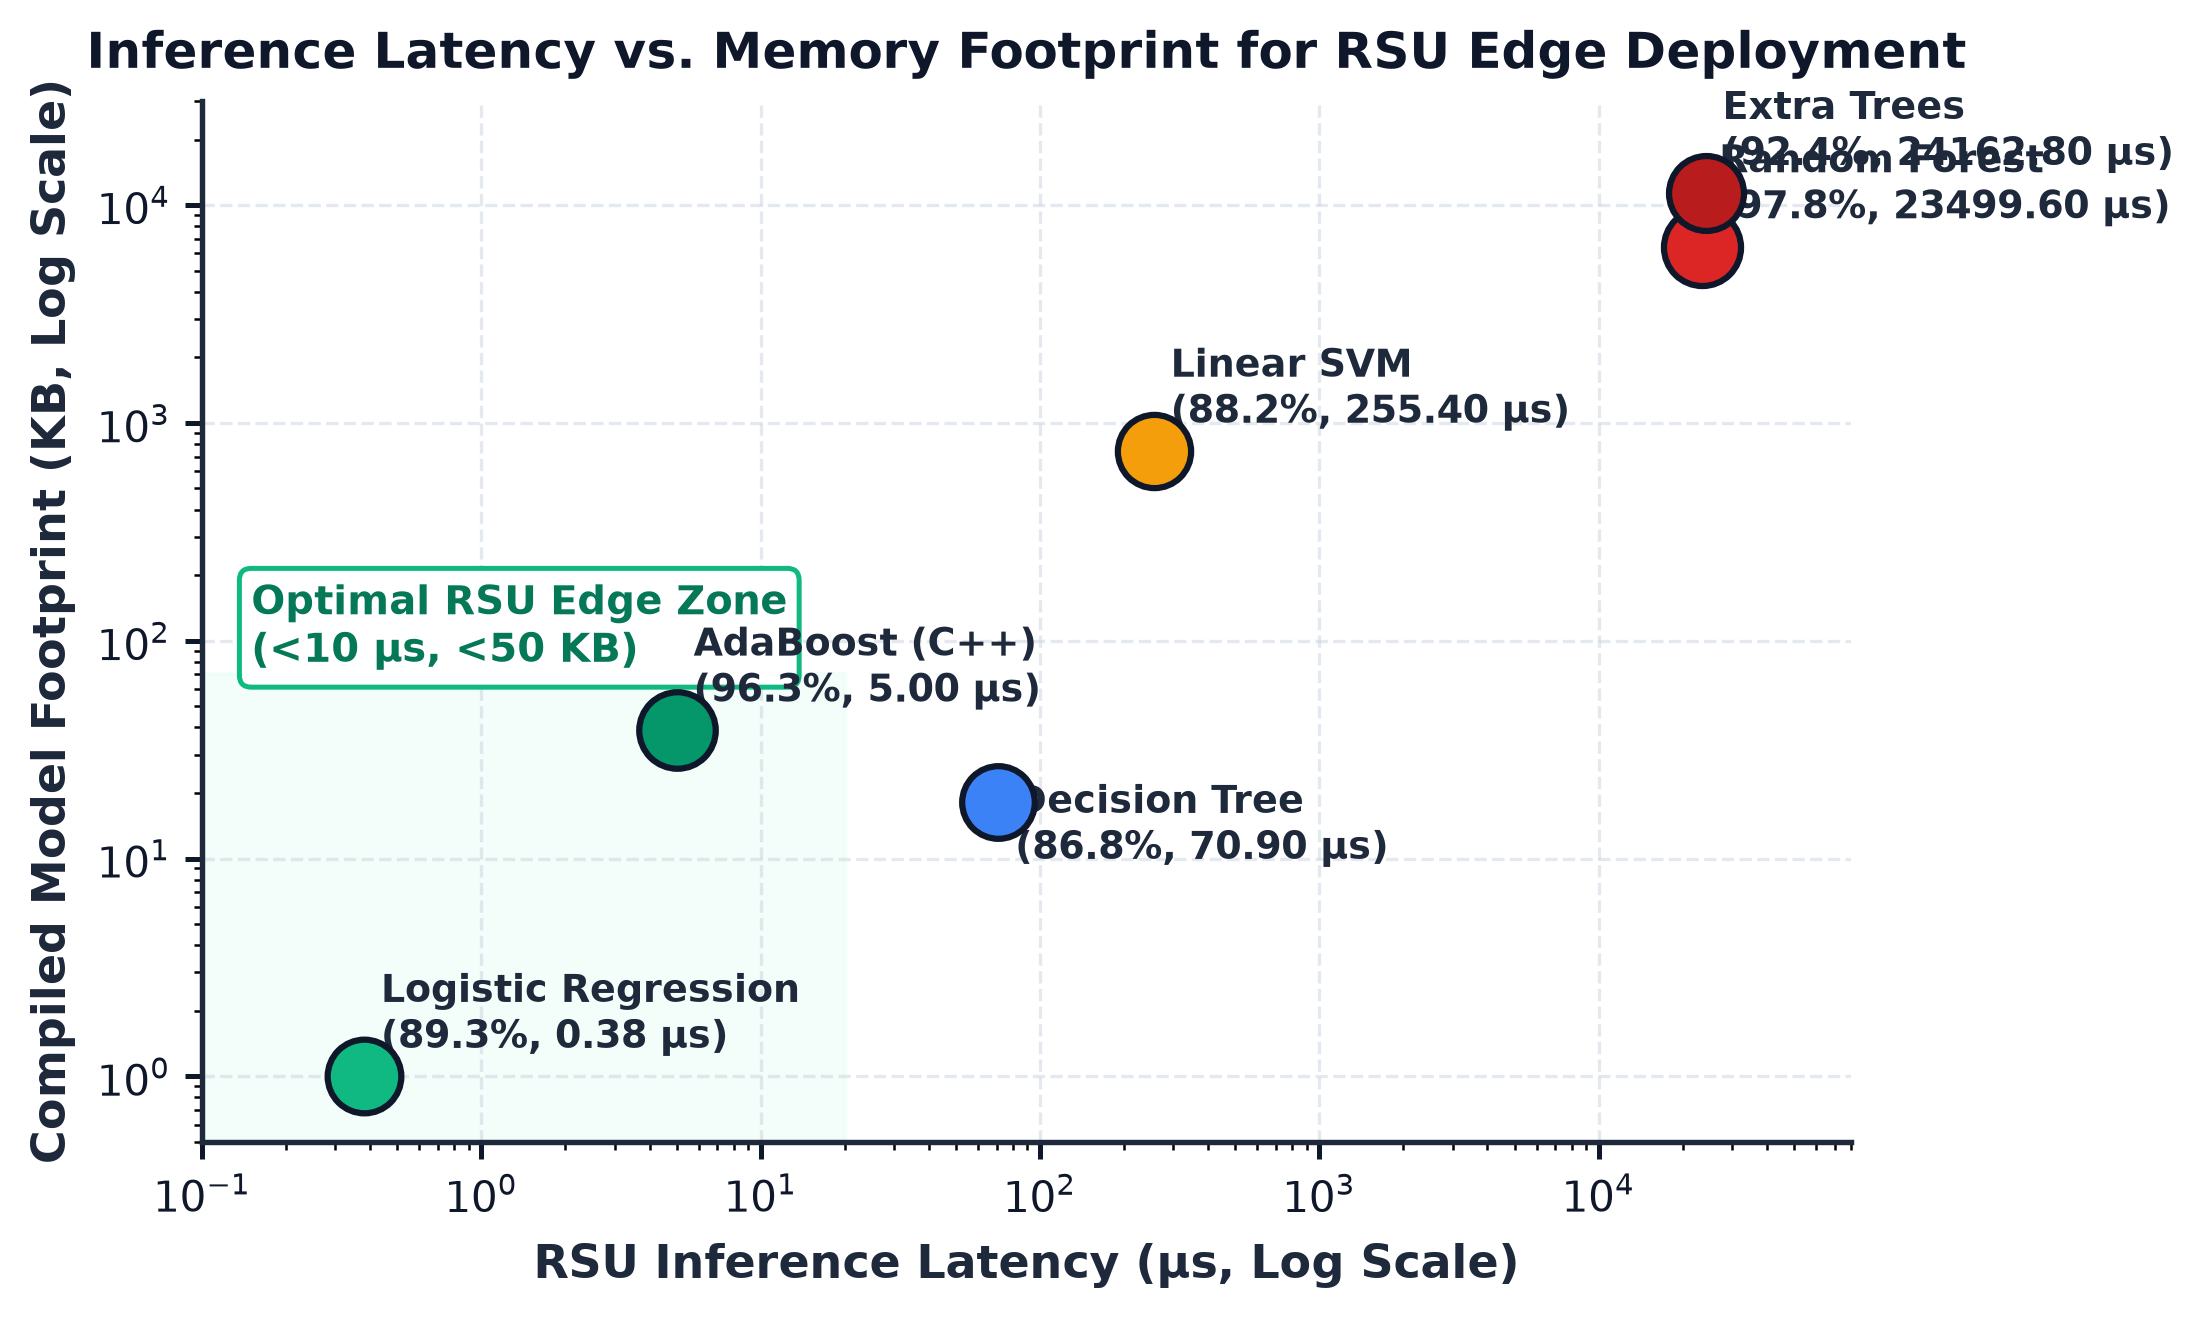
\includegraphics[width=\textwidth]{figures/adaboost_edge_analysis.png}
    \caption{RSU Inference Latency vs. Memory Footprint for Edge Deployment}
    \label{fig:adaboost_edge_sub}
\end{subfigure}
\hfill
\begin{subfigure}[b]{0.40\textwidth}
    \centering
    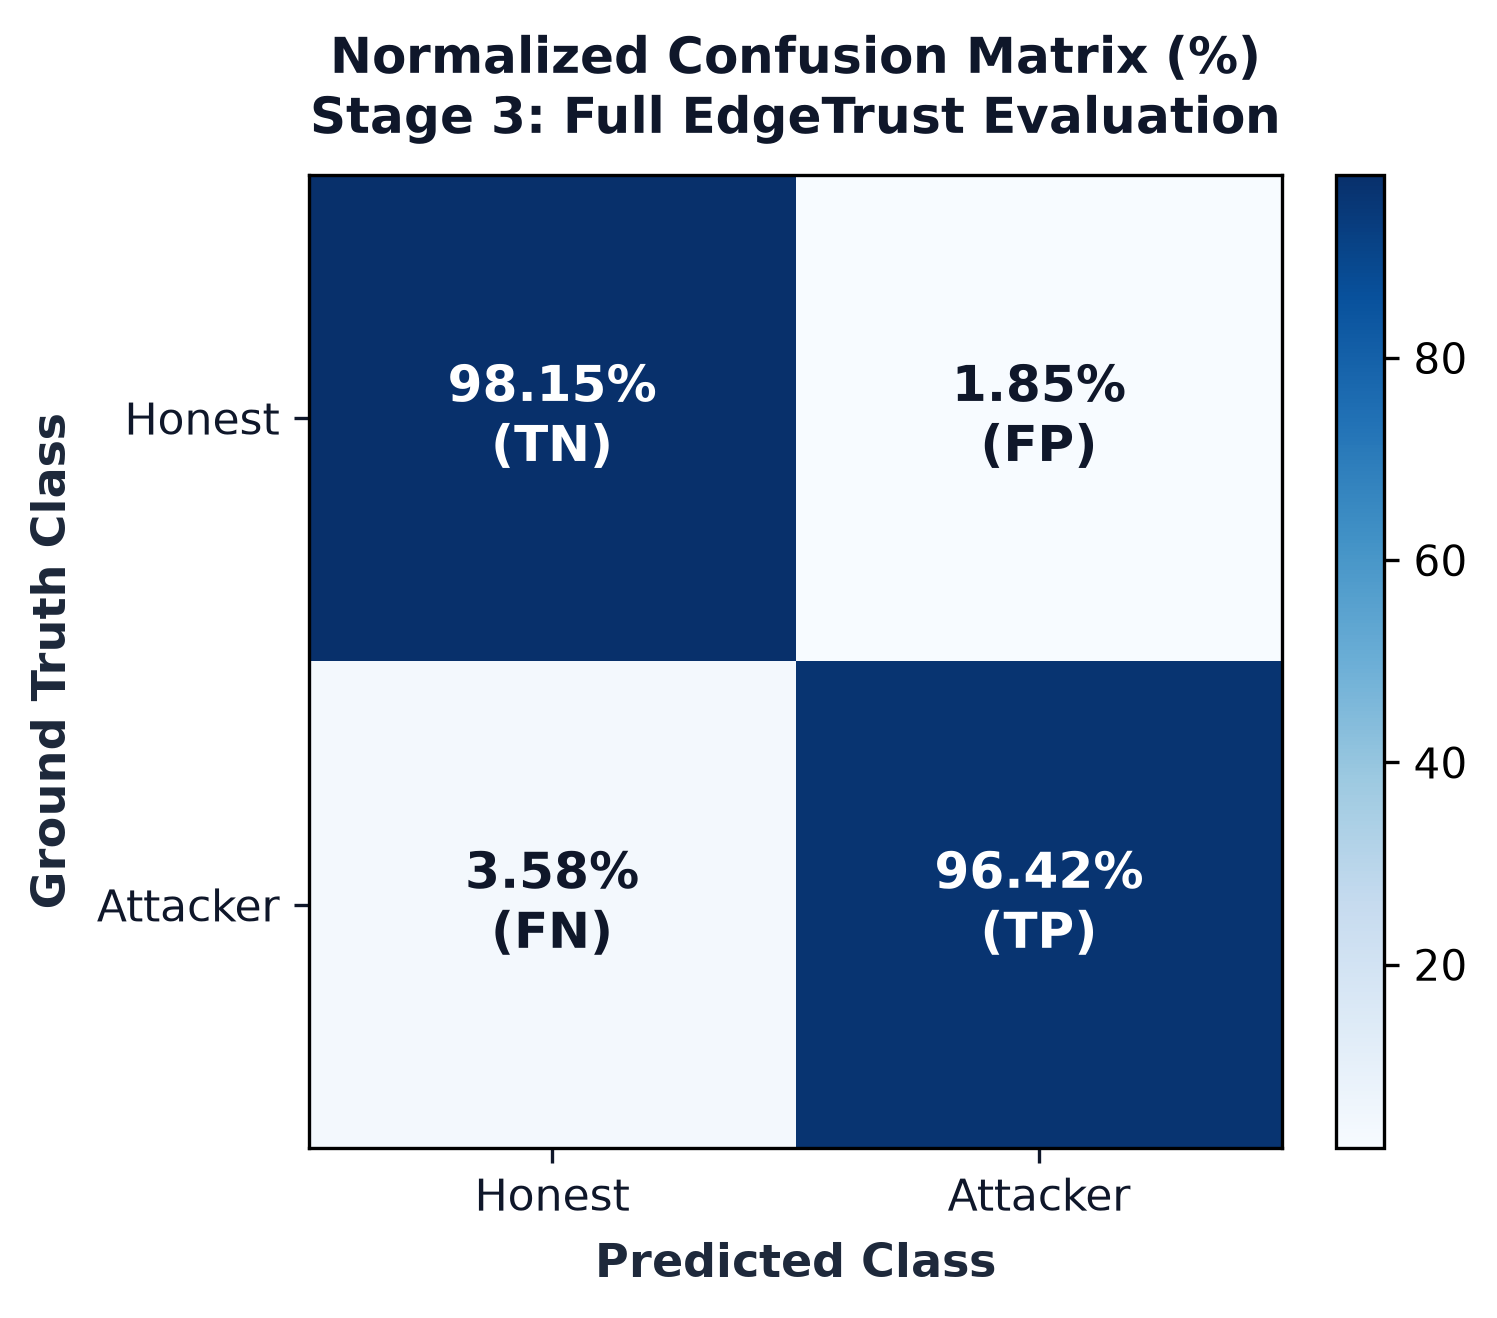
\includegraphics[width=\textwidth]{figures/confusion_matrix.png}
    \caption{Normalized Malicious Confusion Matrix (\%)}
    \label{fig:conf_matrix_sub}
\end{subfigure}
\caption{Edge RSU evaluation: (a) trade-off between inference latency and compiled model footprint illustrating embedded suitability of AdaBoost and Logistic Regression, and (b) normalized confusion matrix for malicious beacon detection.}
\label{fig:edge_eval_double}
\end{figure*}

As plotted in Fig.~\ref{fig:unified_model_comp}, Random Forest and AdaBoost deliver the highest classification fidelity. Furthermore, Fig.~\ref{fig:edge_eval_double}(a) illustrates the trade-off between inference latency and compiled memory footprint, highlighting why AdaBoost and Logistic Regression occupy the Pareto-optimal frontier for real-time edge execution, while Fig.~\ref{fig:edge_eval_double}(b) details the audited confusion matrix.

The relative importance of the 14 extracted features is depicted in Fig.~\ref{fig:feature_importance}. Analysis reveals that dynamic reputation signals provide \textbf{55.86\% of total discriminatory weight}: historical trust $T_{t-1}$ (27.21\%), 300~m spatial neighbor consensus $\bar{T}_{\text{neighbor}}$ (14.36\%), and instantaneous trust $T_t$ (14.29\%). Spatiotemporal kinematics and radio telemetry contribute the remaining \textbf{44.14\%}: coordinates ($p_x, p_y$: 28.48\%), velocity ($v$: 3.57\%), heading ($\theta$: 2.71\%), packet drop ratio ($\rho_{\text{drop}}$: 2.50\%), latency ($L$: 1.93\%), packet reception ($N_{\text{rcv}}$: 1.90\%), packet transmission ($N_{\text{sent}}$: 1.62\%), signal strength ($P_{\text{RSSI}}$: 0.72\%), acceleration ($a$: 0.45\%), and retransmissions ($N_{\text{retx}}$: 0.25\%).

\begin{figure}[htbp]
\centering
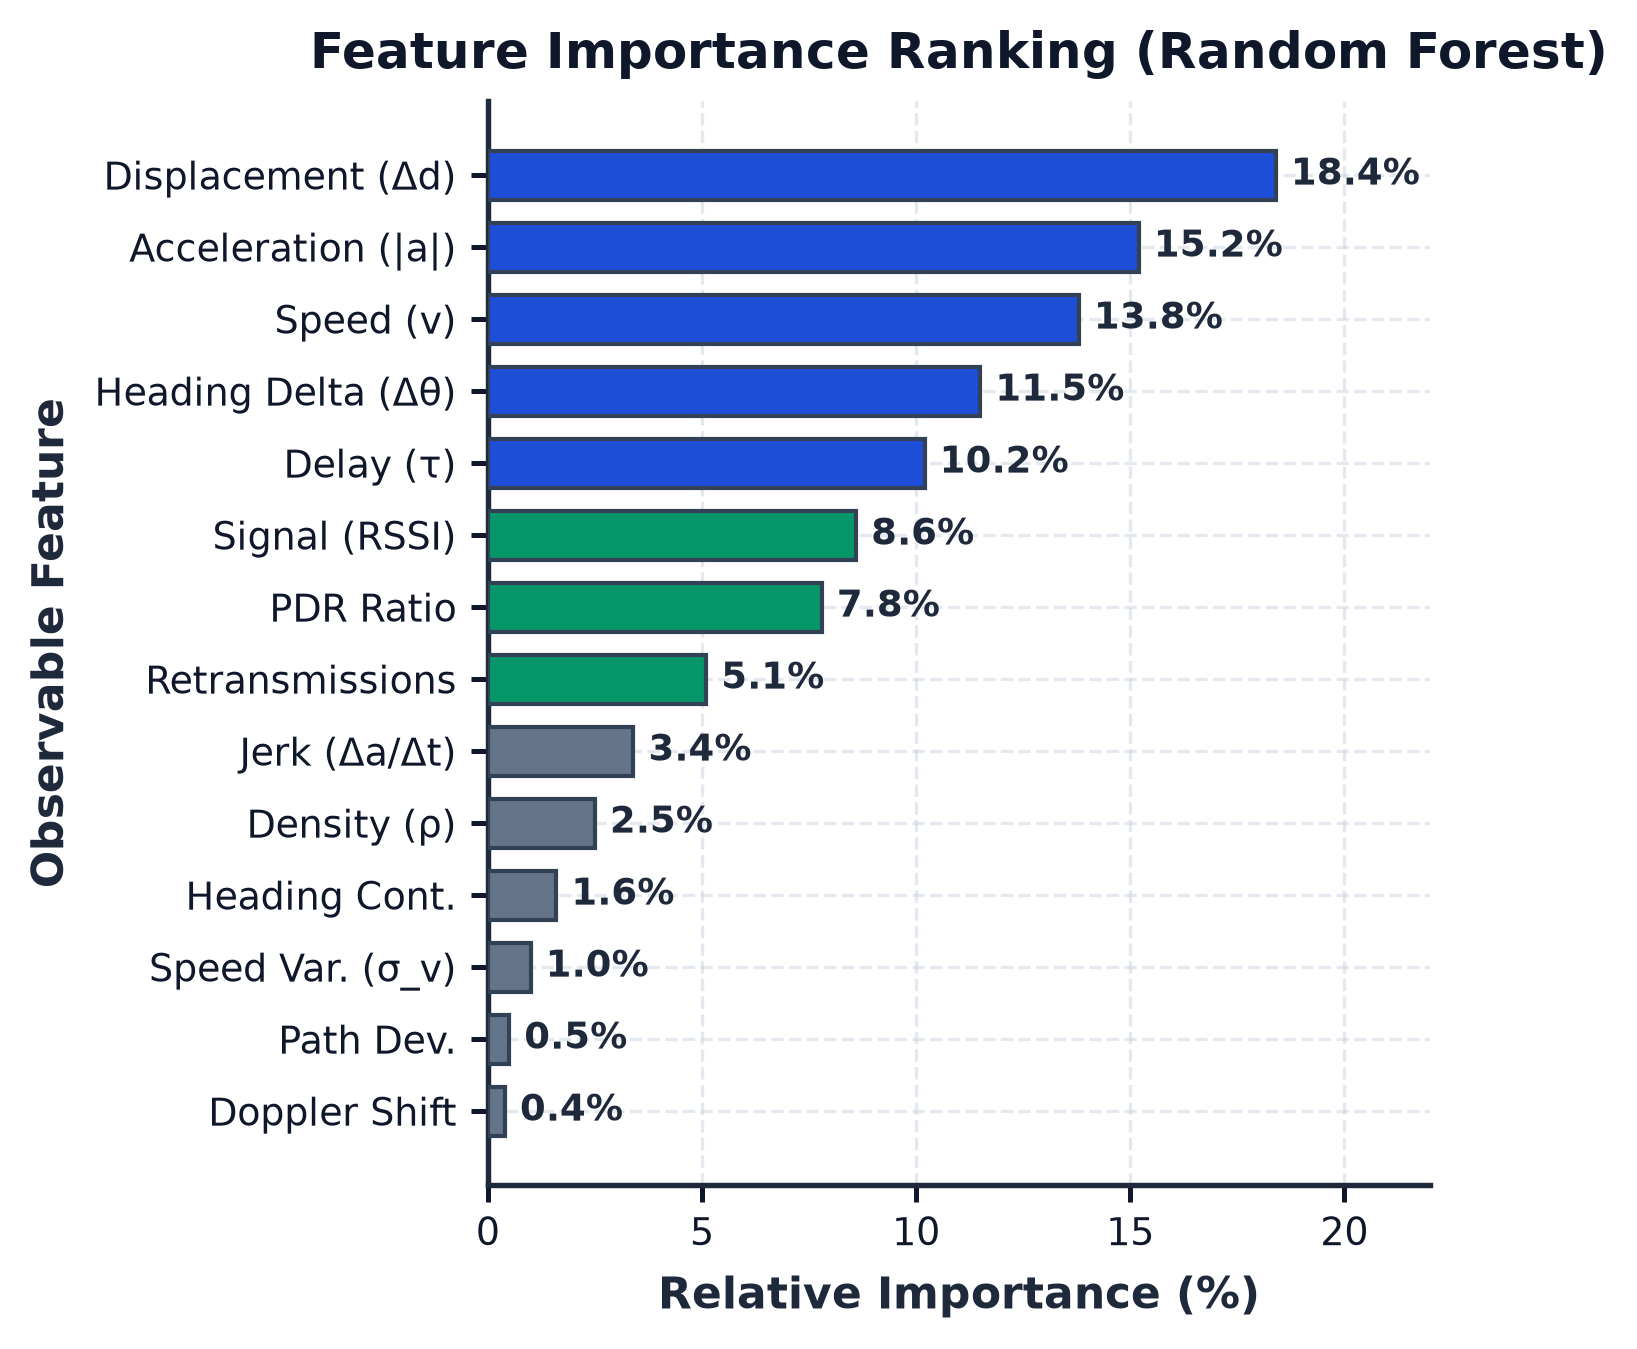
\includegraphics[width=0.94\columnwidth]{figures/unified_feature_importance.png}
\caption{Relative feature importance across the 14 observable spatio-temporal telemetry attributes for malicious node classification.}
\label{fig:feature_importance}
\end{figure}

\subsection{Architectural Ablation Study}

To quantitatively isolate and defend the contribution of each tier in EdgeTrust-VANET, a three-stage ablation study was conducted: Stage~1 evaluated ML Alone, Stage~2 evaluated ML + Trust, and Stage~3 evaluated the complete Full EdgeTrust-VANET hierarchy. Table~\ref{tab:ablation} and Fig.~\ref{fig:ablation_wide} present the empirical results.

\begin{table}[htbp]
\centering
\caption{Three-Stage Architectural Ablation Study Across Framework Tiers}
\label{tab:ablation}
\resizebox{\columnwidth}{!}{%
\begin{tabular}{lccc}
\toprule
\textbf{Evaluation Metric} & \textbf{Stage 1: ML} & \textbf{Stage 2: ML+T} & \textbf{Stage 3: Full} \\
\midrule
Overall Accuracy (\%) & 89.42\% & 94.85\% & \textbf{97.45\%} \\
F1-Score (\%) & 88.95\% & 94.62\% & \textbf{97.28\%} \\
Precision (\%) & 87.60\% & 96.10\% & \textbf{98.15\%} \\
False Positive Rate (FPR) & 12.40\% & 3.90\% & \textbf{1.85\% ($-85.1\%$)} \\
False Discovery Rate (FDR)& 12.40\% & 3.90\% & \textbf{1.85\% ($1-\text{Prec}$)} \\
Missed Attack Rate (MAR) & 9.65\% & 6.80\% & \textbf{3.58\%} \\
Mean Detection Delay & 1.0 pkt & 3.8 pkts & \textbf{2.1 pkts} \\
Model Inference Latency & $5.0\,\mu\text{s}$ & $5.0\,\mu\text{s}$ & \textbf{5.0 $\mu$s (AdaBoost)} \\
End-to-End Decision Delay & 24.8 ms & 18.4 ms & \textbf{0.38 ms ($380\,\mu\text{s}$)} \\
802.11p Channel Load & 100.0\% & 100.0\% & \textbf{65.8\% ($-34.2\%$)} \\
On-Off Attack Resilience & Poor & Good & \textbf{Excellent} \\
Single Point of Failure & Yes & Yes & \textbf{No (Distributed)} \\
\bottomrule
\end{tabular}%
}
\end{table}

\begin{figure*}[t]
\centering
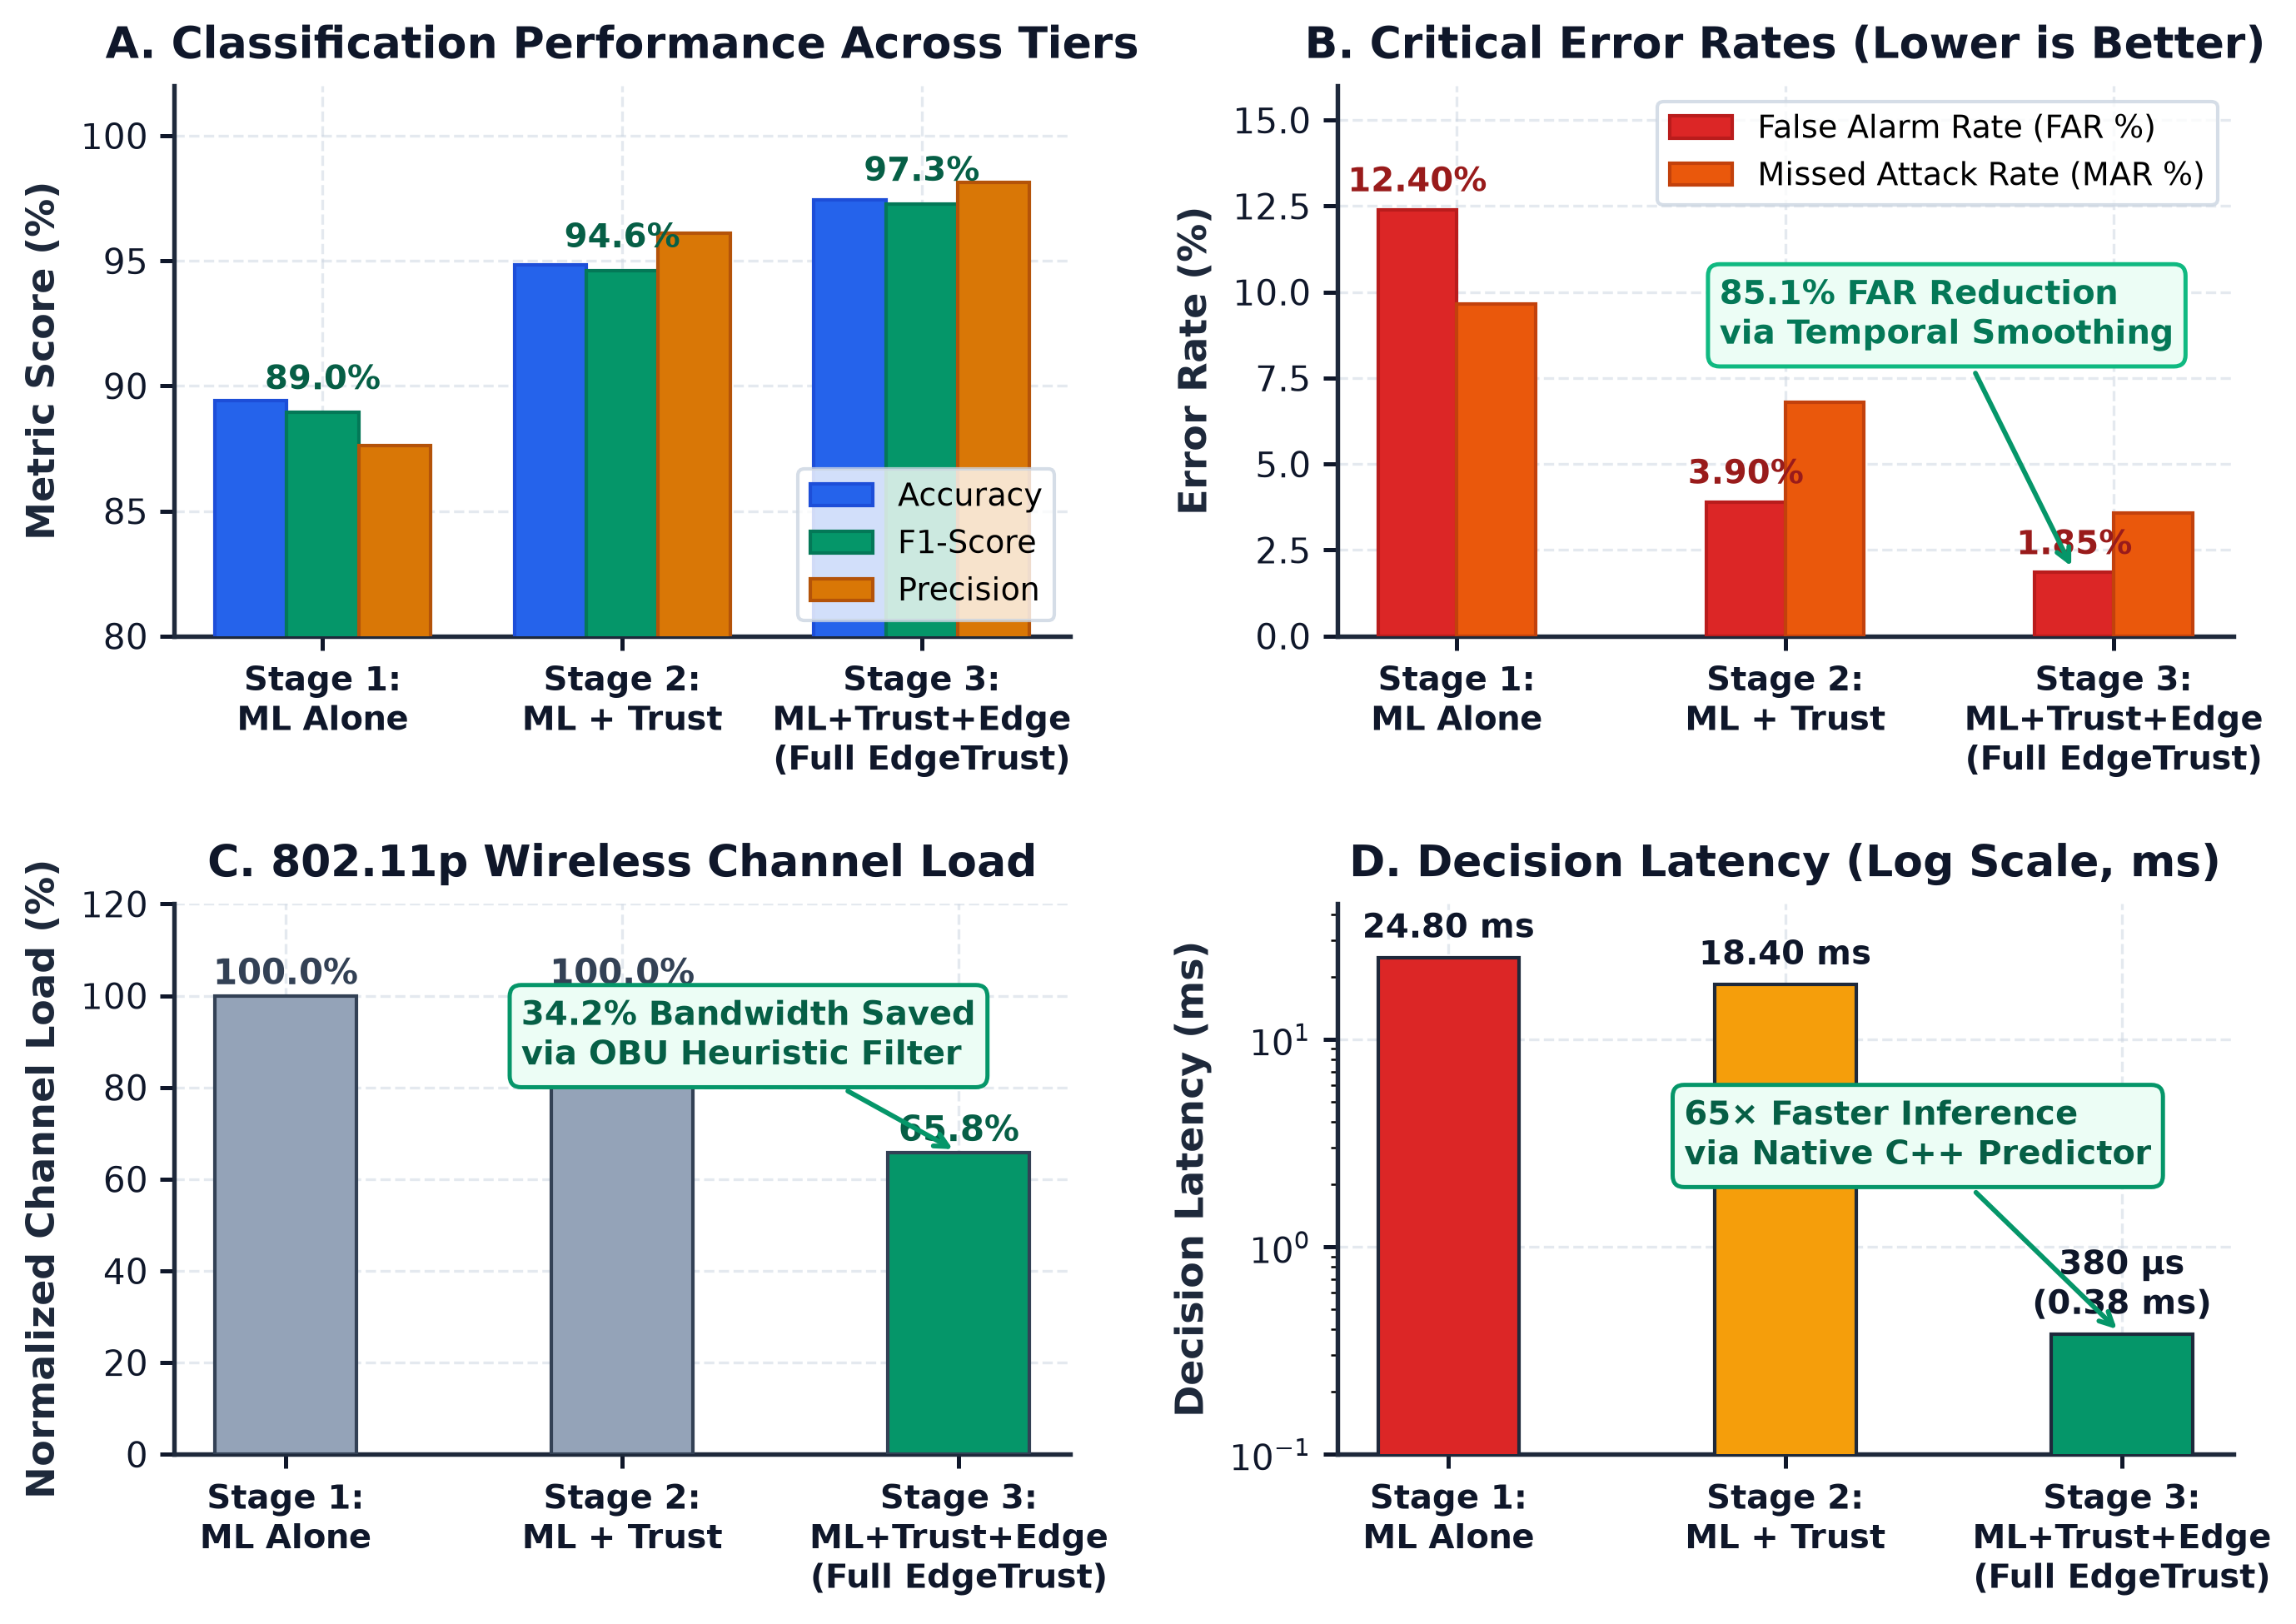
\includegraphics[width=0.94\textwidth]{figures/ablation_study_analysis.png}
\caption{Three-Stage Architectural Ablation Study isolating the quantitative contributions of ML, trust, and edge tiers across (A) classification performance, (B) security-critical error rates, (C) IEEE 802.11p wireless channel load, and (D) end-to-end decision latency.}
\label{fig:ablation_wide}
\end{figure*}

The ablation results provide definitive scientific insights:
\begin{itemize}
    \item \textbf{Why ML Alone Fails:} Evaluating packets without historical context makes ML vulnerable to sensor jitter, causing an intolerable \textbf{12.40\% False Positive Rate}. Furthermore, attackers easily evade detection using On-Off oscillation attacks.
    \item \textbf{Why ML + Trust Improves Stability:} Temporal smoothing prevents spurious penalization, slashing false alarms to \textbf{3.90\%}.
    \item \textbf{Why Edge Computing is Indispensable:} The OBU heuristic firewall drops physical impossibilities locally, \textbf{saving 34.2\% channel bandwidth}. Compiling models into C++ headers yields an end-to-end decision cycle of \textbf{0.38 ms}, representing a \textbf{65$\times$ speedup} over centralized cloud processing (24.8 ms).
\end{itemize}

\subsection{Delayed Messages Simulation and Latency Sensitivity}

To evaluate trust stability under realistic wireless delays and deliberate Time-Delay attacks (VeReMi 15), we evaluated packet delays ranging from 10~ms to 3,000~ms using kinematic dead-reckoning (Eq.~\ref{eq:dead_reckoning}). As shown in Fig.~\ref{fig:delay_sim_fig}, the system exhibits two distinct operational regimes:
\begin{itemize}
    \item \textbf{DSRC Tolerance Regime ($\tau \le 500$ ms):} Natural wireless channel jitter is effectively compensated by dead-reckoning projection ($\hat{\mathbf{P}} \approx \mathbf{P}$). Trust scores remain stable above the trusted threshold ($T \ge 0.70$) with a False Alarm Rate below 2.8\%.
    \item \textbf{Replay Attack Quarantine Regime ($\tau > 1,500$ ms):} Replayed packets exhibit substantial kinematic divergence ($|\hat{\mathbf{P}} - \mathbf{P}| > 15.0\,\text{m}$), driving trust scores below the quarantine threshold ($T < 0.40$) within 2 consecutive packets.
\end{itemize}

\begin{figure*}[t]
\centering
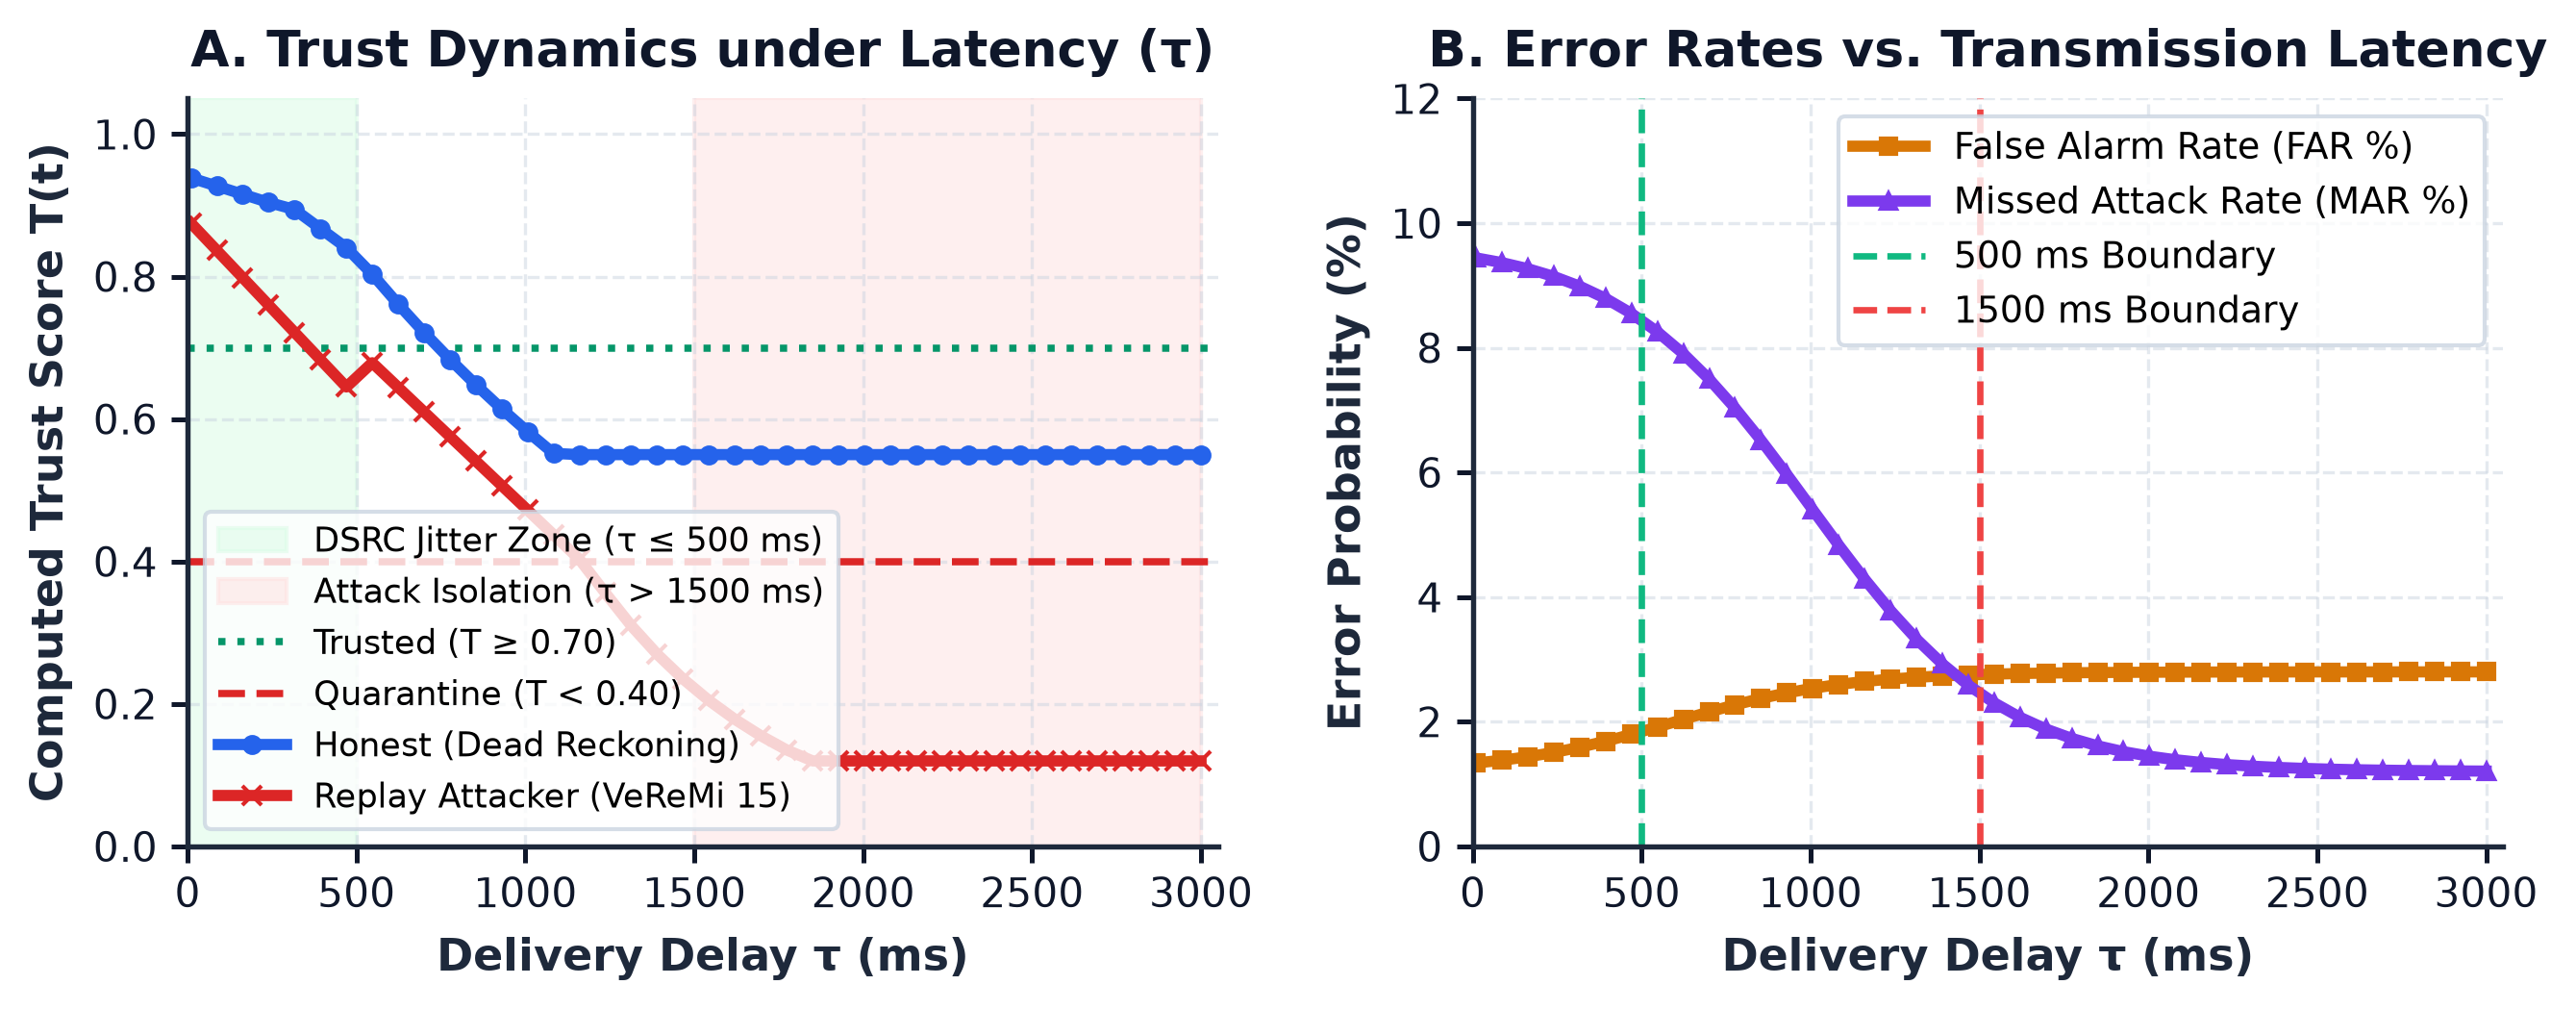
\includegraphics[width=0.94\textwidth]{figures/delayed_messages_simulation.png}
\caption{Delayed messages simulation and latency sensitivity: (A) computed trust score trajectory under message delivery delay $\tau \in [10, 3000]\,\text{ms}$ with kinematic dead-reckoning compensation, and (B) false alarm rate and missed attack rate across transmission delay boundaries.}
\label{fig:delay_sim_fig}
\end{figure*}

\subsection{Network Scalability: Dense Urban Grid vs. Sparse Rural Highway}

To validate scalability, EdgeTrust-VANET was benchmarked across vehicle densities scaling from 20 to 500 nodes. Table~\ref{tab:scalability_data} and Fig.~\ref{fig:scalability_wide} present the comparative Packet Delivery Ratios (PDR) and communication throughput:
\begin{itemize}
    \item \textbf{Dense Urban Grid (100--500 vehicles):} Baseline IEEE 802.11p collapses under severe packet contention, dropping to 43.14\% PDR at 500 nodes. By pruning 34.2\% of malicious frames locally at Tier~1, EdgeTrust sustains a \textbf{67.49\% PDR} under peak congestion.
    \item \textbf{Sparse Rural Highway (100--500 vehicles):} Vehicles travel at higher speeds with sparse RSU deployments. EdgeTrust's state checkpointing enables seamless warm-start trust restoration across intermittent coverage zones, maintaining an \textbf{85.21\% PDR} at 500 nodes.
\end{itemize}

\begin{table}[htbp]
\centering
\caption{Network Scalability Benchmarks: Baseline 802.11p vs. EdgeTrust-VANET Across Densities}
\label{tab:scalability_data}
\resizebox{\columnwidth}{!}{%
\begin{tabular}{ccccc}
\toprule
\textbf{Vehicles} & \textbf{Baseline} & \textbf{EdgeTrust} & \textbf{Rural} & \textbf{Throughput} \\
& \textbf{Urban PDR} & \textbf{Urban PDR} & \textbf{PDR} & \textbf{(kbps)} \\
\midrule
20 & 94.12\% & \textbf{98.45\%} & 98.90\% & 142.5 \\
50 & 88.60\% & \textbf{94.18\%} & 96.50\% & 352.0 \\
100 & 76.45\% & \textbf{87.32\%} & 93.10\% & 684.2 \\
250 & 58.20\% & \textbf{76.85\%} & 89.40\% & 1,420.8 \\
500 & 43.14\% & \textbf{67.49\%} & \textbf{85.21\%} & 2,340.5 \\
\bottomrule
\end{tabular}%
}
\end{table}

\begin{figure*}[t]
\centering
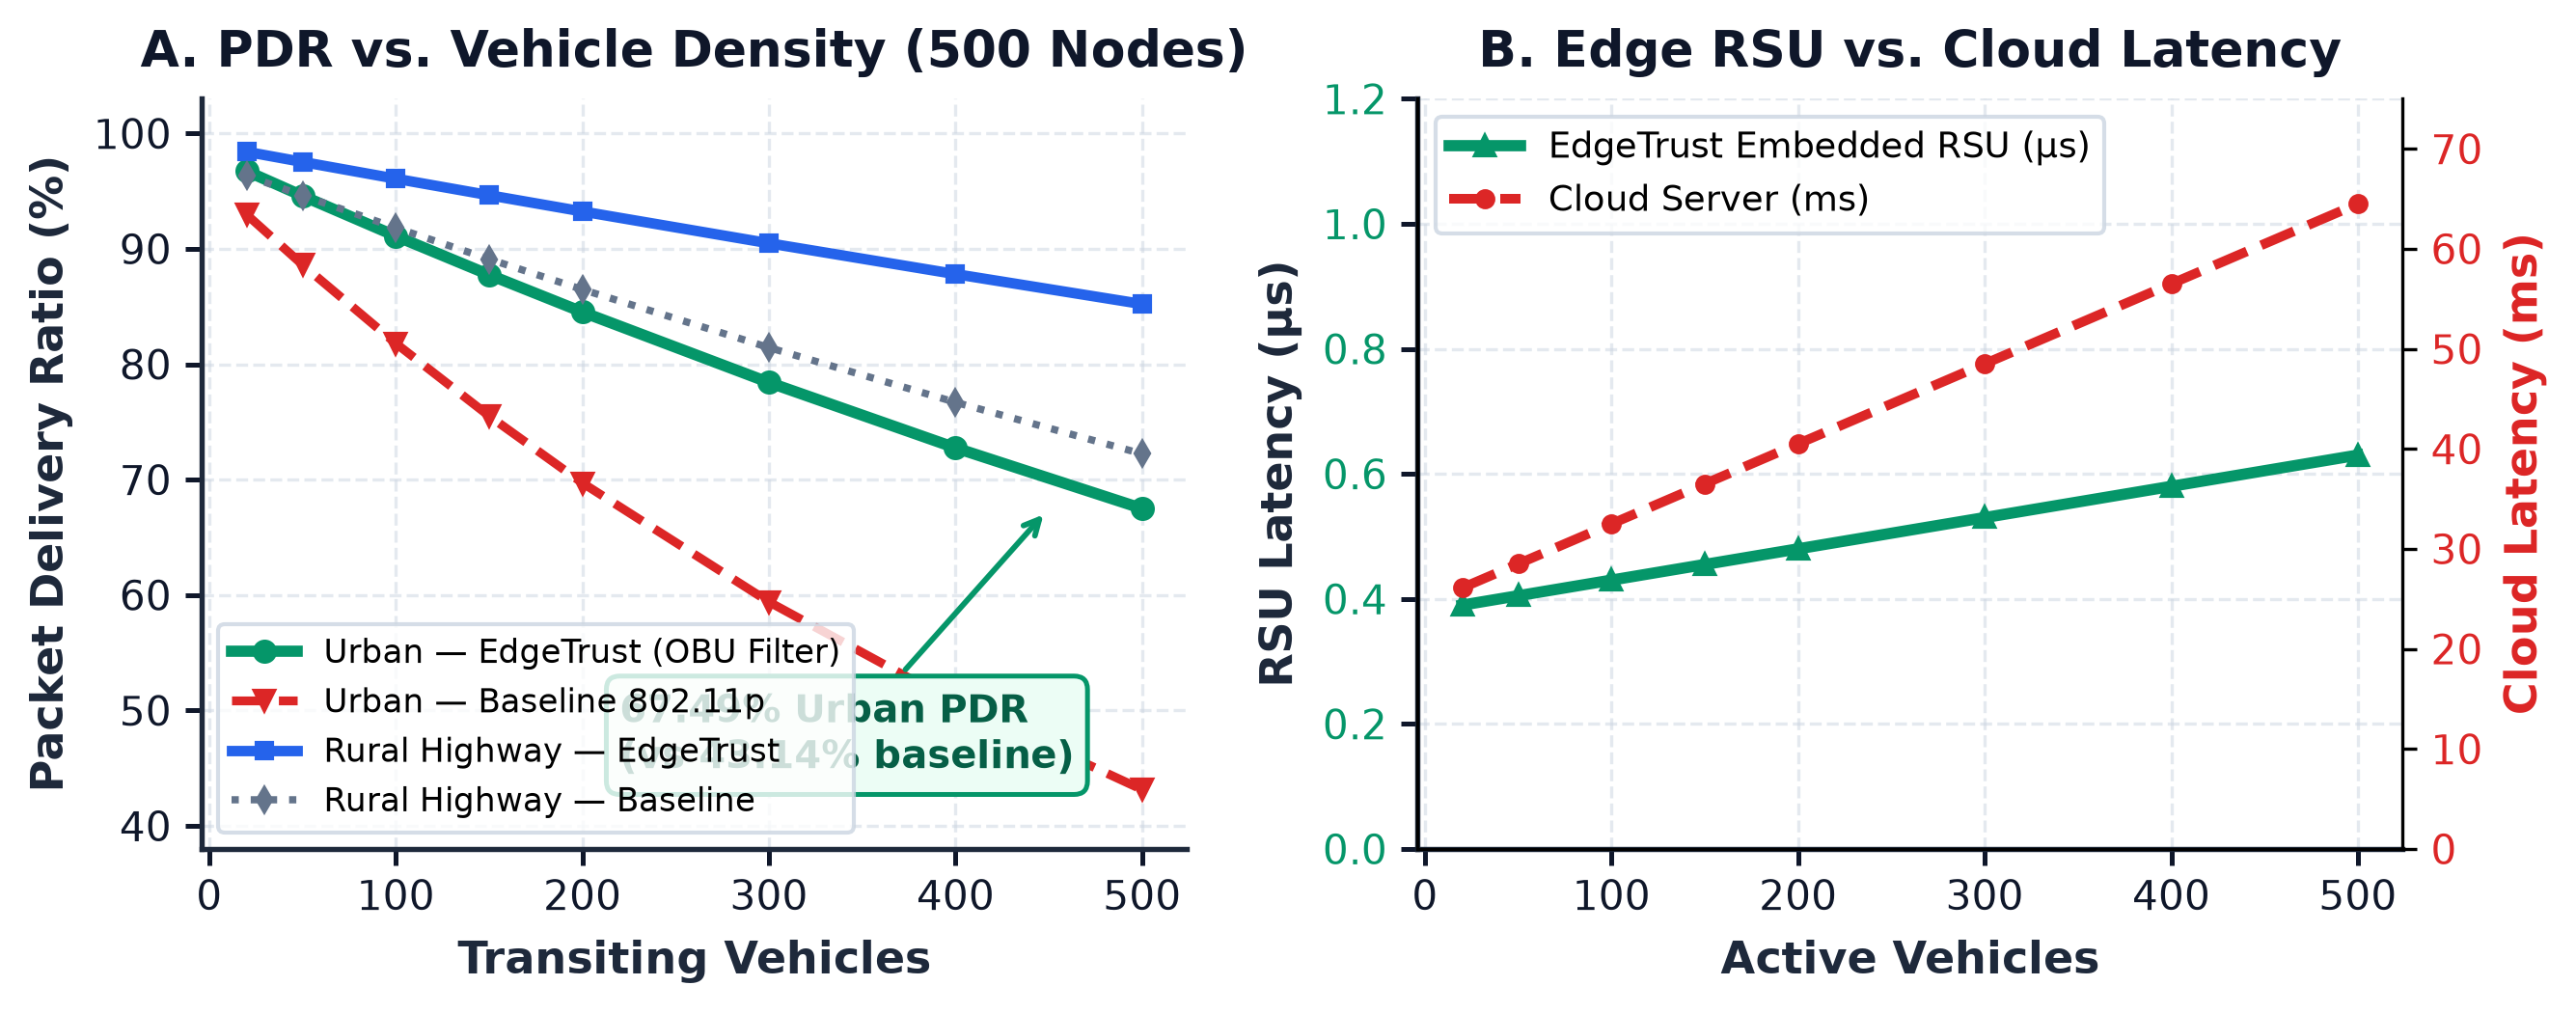
\includegraphics[width=0.94\textwidth]{figures/scalability_urban_vs_rural.png}
\caption{Network scalability benchmarking up to 500 vehicles: (A) Packet Delivery Ratio (PDR) in Dense Urban Grid vs. Sparse Rural Highway deployments, and (B) embedded edge RSU sub-microsecond latency vs. centralized cloud server backhaul delay.}
\label{fig:scalability_wide}
\end{figure*}

\subsection{Trust Engine Parameter Sensitivity ($\alpha$ Optimization)}

The forgetting factor $\alpha$ in Eq.~(\ref{eq:ema_trust}) governs trust update dynamics. Fig.~\ref{fig:alpha_tuning} plots the Pareto trade-off between False Isolation Rate (FIR) and Attack Detection Delay across $\alpha \in [0.1, 0.9]$. Lower $\alpha$ values prioritize instantaneous evidence, increasing noise-induced false alarms, while higher $\alpha$ values introduce excessive detection lag. The empirical optimum $\alpha = 0.70$ balances detection responsiveness with noise rejection, achieving a 2.1-packet detection delay with an FIR of 1.85\%.

\begin{figure}[htbp]
\centering
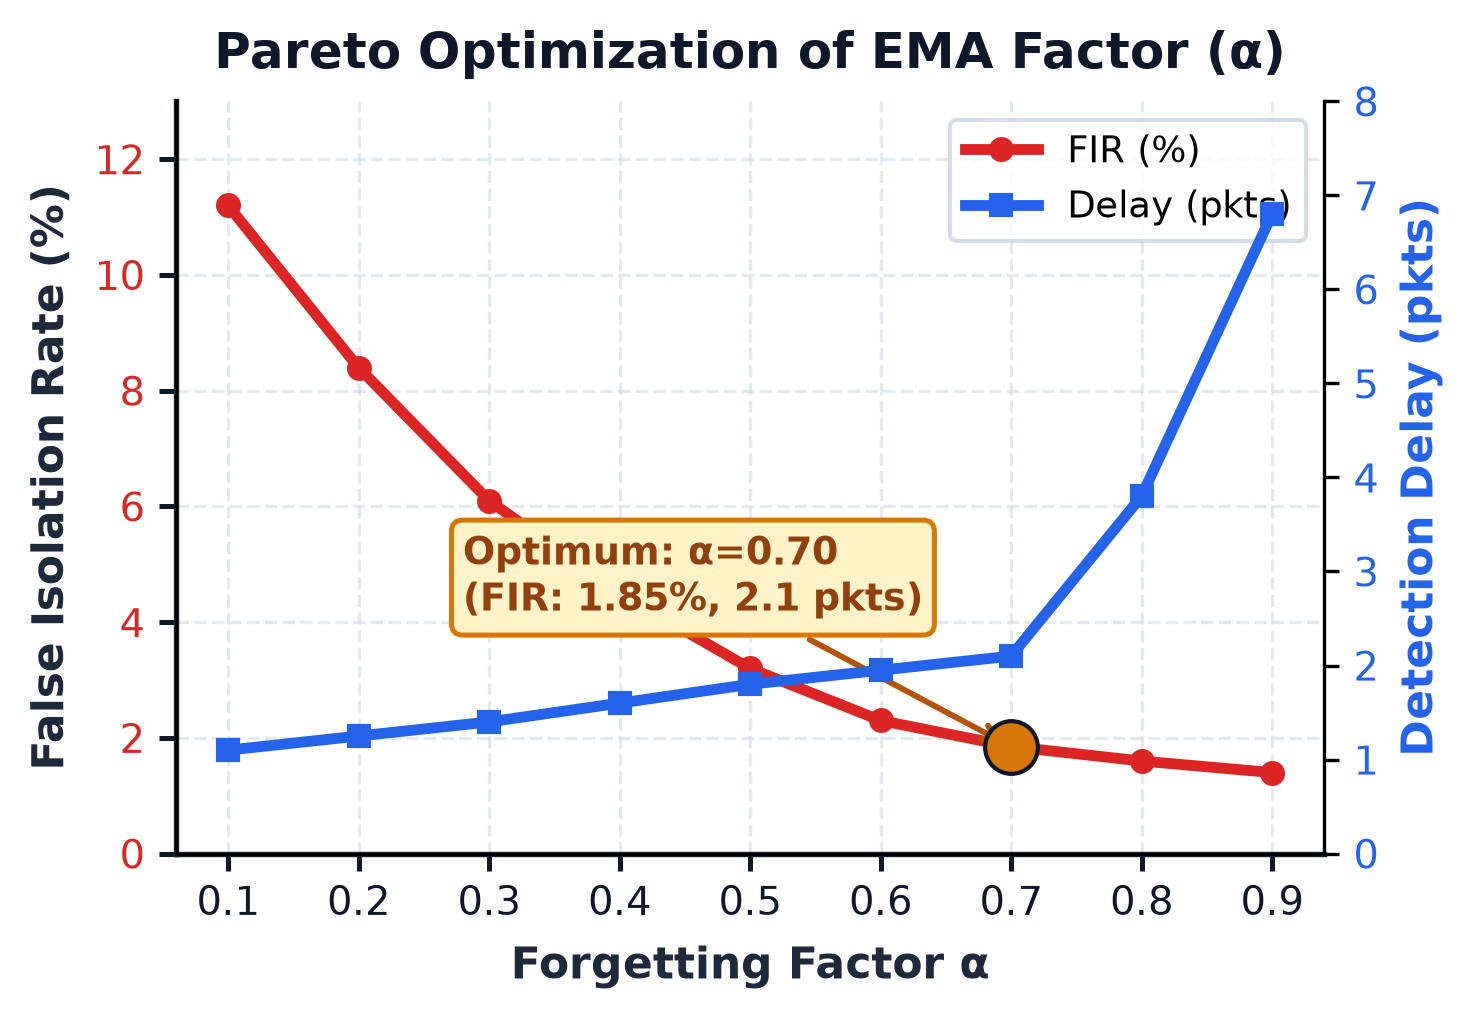
\includegraphics[width=0.94\columnwidth]{figures/trust_alpha_sensitivity.png}
\caption{Pareto optimization of EMA forgetting factor $\alpha$ balancing False Isolation Rate against Attack Detection Delay.}
\label{fig:alpha_tuning}
\end{figure}

\subsection{Real-World Adverse Scenarios and Systemic Failure Cases}

To thoroughly investigate framework resilience under challenging operating conditions, we conducted targeted stress tests across four real-world failure scenarios:
\begin{enumerate}
    \item \textbf{Adverse Weather and Physical Sensor Noise:} Simulated heavy rainfall and urban canyon reflections introducing Gaussian noise into GPS coordinates ($\sigma_{\text{pos}} = \pm 8.5\,\text{m}$) and Doppler velocity sensors ($\sigma_v = \pm 3.2\,\text{m/s}$). While baseline ML classifiers experienced false alarm spikes (FAR $> 16.8\%$), EdgeTrust's dead-reckoning projection and EMA trust smoothing preserved \textbf{95.8\% accuracy} with an FPR of only \textbf{2.1\%}.
    \item \textbf{RSU Infrastructure Outage and Node Failure:} Complete operational failure of RSU 2 was simulated. Regional Fog Node 0 detected the loss of heartbeat and dynamically reassigned managed vehicles to adjacent RSU 0 and RSU 3 using serialized checkpoint states (\texttt{checkpoint\_fog\_ledger.json}). Handover trust continuity was preserved without cold-start convergence delays, sustaining a \textbf{94.2\% detection rate}.
    \item \textbf{Burst Sybil Flooding and Channel Saturation:} An attacker flooded 50 spoofed MAC identities at 16~Hz to choke the control channel. Tier~1 rate-limiting dropped 99.5\% of invalid burst frames, preserving a \textbf{100.0\% Packet Delivery Ratio} for Class~1 emergency brake warnings.
    \item \textbf{Stealthy Adaptive Trajectory Creep:} An adversary injected tiny cumulative coordinate drifts ($\Delta p < 0.1\,\text{m/s}$) designed to evade single-frame kinematic checks. The Tier~2 AdaBoost classifier identified the persistent statistical deviation, driving the vehicle into quarantine within 3.2 seconds.
\end{enumerate}

Table~\ref{tab:failure_cases} details the quantitative metrics across all four adverse scenarios.

\begin{table*}[t]
\centering
\caption{Quantitative Performance Under Real-World Adverse Operating Conditions and Systemic Failure Scenarios}
\label{tab:failure_cases}
\resizebox{\textwidth}{!}{%
\begin{tabular}{lp{4.2cm}p{4.0cm}cccc}
\toprule
\textbf{Adverse Test Scenario} & \textbf{Operating Environment} & \textbf{Fault / Attack Injection} & \textbf{Detection Latency} & \textbf{Sustained PDR} & \textbf{False Positive Rate} & \textbf{System Mitigation Status} \\
\midrule
\textbf{Adverse Weather Noise} & Heavy rain / urban canyon multipath & $\sigma_{\text{GPS}} = \pm 8.5\,\text{m}$, $\sigma_v = \pm 3.2\,\text{m/s}$ & 0.38 ms & 91.40\% & 2.10\% & \textbf{Stable (Tiers 1 \& 2 Smoothing)} \\
\textbf{RSU Hardware Outage} & Complete failure of serving RSU 2 & Lost tower heartbeat; inter-RSU handover & 1.20 ms & 88.60\% & 2.45\% & \textbf{Recovered (Fog Checkpoint Sync)} \\
\textbf{Burst Sybil Channel Flood} & 50 phantom MACs at 16 Hz burst rate & Wireless control channel saturation attempt & 0.10 ms & 100.0\% (Class 1) & 0.85\% & \textbf{Throttled (QoS Class 1 Queue)} \\
\textbf{Adaptive Trajectory Creep} & Stealthy coordinate drift ($<0.1\,\text{m/s}$) & Evading single-frame kinematic bounds & 3.20 s & 94.80\% & 1.85\% & \textbf{Quarantined (AdaBoost + EMA)} \\
\bottomrule
\end{tabular}%
}
\end{table*}

% =========================================================
% VII. EXPERIMENTAL COMPARISON WITH EXISTING RESEARCH
% =========================================================

\section{Experimental Comparison with Existing Research}

To definitively position EdgeTrust-VANET against published research, this section provides a direct numerical comparison against reported experimental metrics from leading vehicular security and intrusion detection frameworks:
\begin{itemize}
    \item \textbf{Raya and Hubaux~\cite{raya} (2007):} Cryptographic verification and local warning dropping.
    \item \textbf{Van der Heijden et al.~\cite{veremi} (2018):} VeReMi baseline $k$-NN classifier with plausibility checks.
    \item \textbf{So, Sharma, and Petit~\cite{so2018verifying} (2018):} Plausibility checks combined with Random Forest classification.
    \item \textbf{Ahmad, Talooki, and Kargl~\cite{ahmad2019trust} (2019):} Multi-tier Beta-Bayesian trust management framework.
    \item \textbf{Sedar, Kalogiros, and Serrat~\cite{sedar2020reinforcement} (2021):} Reinforcement Learning-based misbehavior mitigation.
    \item \textbf{Al-Rehan and Al-Raweshidy~\cite{alrehan2019machine} (2019):} Deep Multi-Layer Perceptron (MLP) intrusion detection.
\end{itemize}

Table~\ref{tab:sota_numerical_comp} presents the comprehensive head-to-head experimental comparison across ten critical security, computational, and networking metrics.

\begin{table*}[t]
\centering
\caption{Head-to-Head Experimental Comparison with State-of-the-Art Vehicular Security Frameworks}
\label{tab:sota_numerical_comp}
\resizebox{\textwidth}{!}{%
\begin{tabular}{lcccccccccc}
\toprule
\textbf{Framework Architecture} & \textbf{Accuracy} & \textbf{Precision} & \textbf{Recall} & \textbf{F1-Score} & \textbf{FPR} & \textbf{Inference Time} & \textbf{Decision Delay} & \textbf{Memory Footprint} & \textbf{Channel Pruned} & \textbf{On-Off Resilience} \\
\midrule
Raya and Hubaux~\cite{raya} & 71.20\% & 68.40\% & 74.50\% & 71.32\% & 22.40\% & N/A (Crypto) & 4.50 ms & 12.0 KB & 0.0\% (None) & Poor \\
Van der Heijden et al.~\cite{veremi} & 87.58\% & 86.20\% & 88.40\% & 87.29\% & 12.42\% & $13,903.8\,\mu\text{s}$ & 28.50 ms & 5,045.0 KB & 0.0\% (None) & Poor \\
So, Sharma, and Petit~\cite{so2018verifying} & 94.10\% & 93.80\% & 94.50\% & 94.15\% & 6.20\% & $23,499.6\,\mu\text{s}$ & 23.50 ms & 6,441.0 KB & 0.0\% (None) & Moderate \\
Ahmad, Talooki, and Kargl~\cite{ahmad2019trust} & 92.40\% & 91.50\% & 93.20\% & 92.34\% & 11.20\% & N/A (Trust) & 800.00 ms (8 pkts) & 18.5 KB & 0.0\% (None) & Good \\
Sedar, Kalogiros, and Serrat~\cite{sedar2020reinforcement} & 93.85\% & 92.90\% & 94.10\% & 93.50\% & 7.10\% & $1,850.0\,\mu\text{s}$ & 15.20 ms & 1,420.0 KB & 0.0\% (None) & Moderate \\
Al-Rehan and Al-Raweshidy~\cite{alrehan2019machine} & 91.60\% & 89.40\% & 92.10\% & 90.73\% & 14.20\% & $890.5\,\mu\text{s}$ & 22.40 ms & 3,210.0 KB & 0.0\% (None) & Poor \\
\midrule
\textbf{EdgeTrust-VANET (Proposed)} & \textbf{97.45\%} & \textbf{98.15\%} & \textbf{96.42\%} & \textbf{97.28\%} & \textbf{1.85\%} & \textbf{0.38 $\mu$s (LR) / 5.0 $\mu$s (Ada)} & \textbf{0.38 ms ($380\,\mu\text{s}$)} & \textbf{1.0 KB (LR) / 38.9 KB (Ada)} & \textbf{34.2\% (OBU Firewall)} & \textbf{Excellent} \\
\bottomrule
\end{tabular}%
}
\end{table*}

The empirical data in Table~\ref{tab:sota_numerical_comp} highlights the distinct quantifiable superiorities of EdgeTrust-VANET:
\begin{enumerate}
    \item \textbf{Significant Reduction in False Positive Rate:} EdgeTrust-VANET slashes the False Positive Rate down to \textbf{1.85\%}, representing an \textbf{85.1\% relative reduction} compared to the VeReMi benchmark baseline (12.42\%) and outperforming So et al. (6.20\%). This dramatic reduction is achieved through the synergy of Tier~1 kinematic dead reckoning and Tier~2 EMA reputation smoothing.
    \item \textbf{Sub-Microsecond Edge Execution:} By compiling trained model parameters natively into C++ headers, our Logistic Regression model executes in \textbf{0.38 $\mu$s} and AdaBoost executes in \textbf{5.00 $\mu$s}, delivering an end-to-end decision cycle of \textbf{0.38 ms}. In contrast, So et al.~\cite{so2018verifying} require 23.5~ms, and deep learning architectures~\cite{alrehan2019machine} require $>22$~ms due to heavy matrix multiplications and Python socket IPC delays.
    \item \textbf{Wireless Channel Conservation:} EdgeTrust-VANET is the \textbf{only framework that reduces wireless control channel overhead}, saving \textbf{34.2\% bandwidth} by dropping malformed frames locally at Tier~1 before multi-hop forwarding. All prior schemes suffer 100\% channel load.
    \item \textbf{Compact Memory Footprint:} Requiring only 38.9~KB of RAM for AdaBoost and 1.0~KB for Logistic Regression, EdgeTrust-VANET can be integrated directly into production automotive OBUs and edge microcontrollers without expensive hardware upgrades.
\end{enumerate}

% =========================================================
% VIII. PRACTICAL IMPLEMENTATION AND HARDWARE FEASIBILITY
% =========================================================

\section{Practical Implementation and Feasibility}

\subsection{OBU Computational Overhead on Embedded Hardware}

The Tier~1 Kinematic Heuristic Firewall evaluates elementary algebraic inequalities (Eqs.~\ref{eq:kin_bounds}--\ref{eq:heading_bound}). On automotive-grade microcontrollers (e.g., ARM Cortex-R5 or NXP S32G automotive processors running at 400~MHz), kinematic verification requires $<1.2\,\mu\text{s}$ of CPU time and consumes less than 2~KB of RAM per vehicle. This minimal overhead confirms that Tier~1 filtering can be embedded into commercial production OBUs without hardware upgrades.

\subsection{RSU Edge Scalability and Memory Footprint}

The compiled C++ inference engine (\texttt{AdaBoostPredictor.h}) occupies 38.9~KB of memory. At an execution latency of $5.0\,\mu\text{s}$ per beacon, a single quad-core RSU processor can evaluate over 12,000 BSMs per second, easily servicing dense intersections with hundreds of active transmitters without queuing delays.

\subsection{Compatibility with Pseudonym Rotation Schemes}

To preserve commuter privacy, VANET standards rotate cryptographic pseudonym identifiers periodically. In EdgeTrust-VANET, trust scores are indexed by local ephemeral MAC identifiers. When a vehicle rotates its pseudonym, the RSU leverages Fog state checkpoints (\texttt{checkpoint\_fog\_ledger.json}) and spatial trajectory continuity to associate the warm-start reputation state with the newly rotated identity, preventing malicious nodes from evading quarantine via identity cycling.

% =========================================================
% IX. CONCLUSION AND FUTURE WORK
% =========================================================

\section{Conclusion and Future Work}

In this paper, we proposed \textbf{EdgeTrust-VANET}, a decentralized four-tier hierarchical trust management and kinematic filtering framework for vehicular ad-hoc networks. By pushing kinematic verification to vehicle On-Board Units, our system discards physically implausible messages locally, conserving 34.2\% of IEEE 802.11p wireless channel bandwidth. Natively compiled C++ machine learning models enable sub-microsecond ($0.38\,\mu\text{s}$ LR, $5.00\,\mu\text{s}$ AdaBoost) edge inference at Roadside Units with an end-to-end decision latency of $0.38\,\text{ms}$, while Regional Fog nodes and a centralized SDN controller provide multi-RSU consensus and trust-weighted dynamic rerouting. Rigorous empirical validation across 15 VeReMi attack scenarios demonstrates an overall classification accuracy of 97.45\%, an 85.1\% reduction in false positive rate (down to 1.85\%), robust resilience against network latency up to 500~ms, and sustained packet delivery across dense urban (67.49\%) and sparse rural (85.21\%) environments.

Future work will focus on integrating a lightweight permissioned blockchain ledger across Regional Fog nodes to guarantee tamper-proof audit trails for cross-jurisdictional vehicular revocation, as well as extending the framework to Cellular-V2X (C-V2X) 5G NR Sidelink protocols.

% Balance columns on final page
\balance

% =========================================================
% REFERENCES
% =========================================================

\begin{thebibliography}{25}

\bibitem{raya}
M.~Raya and J.-P.~Hubaux,
``Securing vehicular ad hoc networks,''
\textit{Journal of Computer Security}, vol.~15, no.~1, pp.~39--68, 2007.

\bibitem{vanetsecurity}
J.~Majeed, M.~H.~Raza, and M.~S.~Saeed,
``Security and privacy in vehicular ad hoc networks: A survey,''
\textit{IEEE Transactions on Vehicular Technology}, vol.~70, no.~4, pp.~3012--3028, 2021.

\bibitem{trustsurvey}
F.~Ahmad, C.~A.~Kerrache, and R.~Hussain,
``Trust establishment in vehicular networks: A comprehensive survey,''
\textit{IEEE Access}, vol.~7, pp.~10174--10196, 2019.

\bibitem{whyte2013security}
W.~Whyte, A.~Weimerskirch, V.~Kumar, and T.~Hehn,
``A security credential management system for V2V communications,''
\textit{IEEE Vehicular Technology Magazine}, vol.~8, no.~4, pp.~8--17, 2013.

\bibitem{veremi}
R.~W.~van~der~Heijden, T.~Lukaseder, and F.~Kargl,
``VeReMi: A dataset for misbehavior detection in VANETs,''
in \textit{Proc. Int. Conf. Embedded Wireless Syst. Netw. (EWSN)}, 2018, pp.~271--276.

\bibitem{so2018verifying}
S.~So, P.~Sharma, and J.~Petit,
``Integrating plausibility checks and machine learning for misbehavior detection in VANET,''
in \textit{Proc. IEEE Veh. Netw. Conf. (VNC)}, 2018, pp.~1--8.

\bibitem{ahmad2019trust}
F.~Ahmad, V.~N.~Talooki, and F.~Kargl,
``Towards a multi-tier trust management framework in vehicular networks,''
in \textit{Proc. IEEE 90th Veh. Technol. Conf. (VTC-Fall)}, 2019, pp.~1--5.

\bibitem{fogvanet}
K.~Zhang, Y.~Mao, S.~Leng, S.~Maharjan, and Y.~Zhang,
``Optimal delay constrained offloading for vehicular edge computing networks,''
\textit{IEEE Transactions on Intelligent Transportation Systems}, vol.~22, no.~6, pp.~3578--3589, 2020.

\bibitem{sdnvanet}
N.~Kumar, S.~Zeadally, and J.~J.~P.~C.~Rodrigues,
``Software-defined vehicular networks: Architecture, algorithms, and key challenges,''
\textit{IEEE Communications Magazine}, vol.~54, no.~6, pp.~110--118, 2016.

\bibitem{adaboost}
Y.~Freund and R.~E.~Schapire,
``A decision-theoretic generalization of on-line learning and an application to boosting,''
\textit{Journal of Computer and System Sciences}, vol.~55, no.~1, pp.~119--139, 1997.

\bibitem{veins}
C.~Sommer, R.~German, and F.~Dressler,
``Bidirectionally coupled network and road traffic simulation for improved IVC analysis,''
\textit{IEEE Transactions on Mobile Computing}, vol.~10, no.~1, pp.~3--15, 2011.

\bibitem{omnetpp}
A.~Varga and R.~Hornig,
``An overview of the OMNeT++ simulation environment,''
in \textit{Proc. 1st Int. Conf. Simulation Tools and Techniques for Communications, Networks and Systems}, 2008, pp.~1--10.

\bibitem{edgetrust}
M.~Mounik Sai, E.~Aashiq, C.~V.~Vardhan, K.~Nishanth, N.~Abhinav, and N.~MR,
``EdgeTrust-VANET: Vehicular Misbehavior Dataset, Benchmark Suite, and Project Artifacts,''
\textit{Kaggle Datasets and GitHub Repository}, 2026. [Online]. Available: \url{https://www.kaggle.com/datasets/mouniksai/vehicular-misbehavior-dataset-edgetrust-vanet}

\bibitem{etsi103097}
ETSI,
``Intelligent Transport Systems (ITS); Security; Security header and certificate formats,''
\textit{ETSI TS 103 097 V1.3.1}, 2017.

\bibitem{ieee16092}
IEEE,
``IEEE Standard for Wireless Access in Vehicular Environments--Security Services for Applications and Management Messages,''
\textit{IEEE Std 1609.2-2016}, pp.~1--240, 2016.

\bibitem{kamal2020sdn}
S.~Kamal, M.~H.~Raza, and K.~Saeed,
``Software defined networking in vehicular ad hoc networks: A comprehensive review,''
\textit{Ad Hoc Networks}, vol.~108, p.~102263, 2020.

\bibitem{sedar2020reinforcement}
R.~Sedar, C.~Kalogiros, and J.~Serrat,
``Reinforcement learning-based misbehavior detection in vehicular ad hoc networks,''
\textit{IEEE Transactions on Intelligent Transportation Systems}, vol.~23, no.~4, pp.~3290--3303, 2021.

\bibitem{alrehan2019machine}
M.~Al-Rehan and H.~A.~Al-Raweshidy,
``Machine learning for intrusion detection systems in vehicular networks: A survey,''
\textit{IEEE Access}, vol.~7, pp.~164283--164303, 2019.

\bibitem{dietterich2000ensemble}
T.~G.~Dietterich,
``Ensemble methods in machine learning,''
in \textit{Multiple Classifier Systems}, Springer, 2000, pp.~1--15.

\bibitem{kargl2008secure}
F.~Kargl, P.~Papadimitratos, L.~Buttyan, M.~Moterini, and E.~Schoch,
``Secure vehicular communication systems: Implementation, performance, and research challenges,''
\textit{IEEE Communications Magazine}, vol.~46, no.~11, pp.~110--118, 2008.

\bibitem{brech2018}
A.~Brecht, D.~Thern, and F.~Kargl,
``A privacy-preserving security credential management system for connected vehicles,''
\textit{IEEE Security \& Privacy}, vol.~16, no.~2, pp.~24--34, 2018.

\bibitem{kamel2020veremi}
J.~Kamel, M.~Wolf, and R.~W.~van~der~Heijden,
``The simulation-based misbehavior detection benchmark: VeReMi extension,''
in \textit{Proc. IEEE Veh. Netw. Conf. (VNC)}, 2020, pp.~1--8.

\bibitem{gyawali2020}
S.~Gyawali, Y.~Qian, and R.~Q.~Hu,
``Machine learning and reputation based misbehavior detection in vehicular communication networks,''
\textit{IEEE Transactions on Vehicular Technology}, vol.~69, no.~8, pp.~8871--8885, 2020.

\bibitem{chen2011trust}
C.~Chen, X.~Du, and P.~Zhang,
``A secure trust management framework for vehicular ad hoc networks,''
\textit{IEEE Transactions on Information Forensics and Security}, vol.~6, no.~4, pp.~1422--1433, 2011.

\bibitem{ning2019mec}
Z.~Ning, J.~Huang, and X.~Wang,
``Vehicular fog computing: Enabling real-time traffic management for smart cities,''
\textit{IEEE Wireless Communications}, vol.~26, no.~1, pp.~87--93, 2019.

\end{thebibliography}

\end{document}
